\documentclass[dissertation,appendsingle]{MSUstyle}
%
%  Created by Seth Humphries 
%  Update and maintained by Prof. Mark Owkes mark.owkes@montana.edu
% 
%%    Copyright (c) 2007-2012 Seth D. Humphries
%%    This work is licensed under the Creative Commons
%%    Attribution-Noncommercial-Share Alike 3.0 License. To view a copy
%%    of this license, visit http://creativecommons.org/licenses/by-nc-sa/3.0/;
%%    or, (b) send a letter to Creative Commons, 171 2nd Street, Suite
%%    300, San Francisco, California, 94105, USA. 
%
%  Version 2.0, check for periodic updates on the bitbucket repository
%
% DEFAULTS --------------------
% The default options are as follows:
%   \documentclass[12pt,letterpaper,oneside,openright,%
%       doublespaced,normalmargins,dissertation,final,numreset]{MSUstyle}
%
% default options do not need to be entered. Defaults will generate a document 
% that conforms to the MSU Electronic Thesis/Dissertation  (ETD) guidelines. 
%
% MASTERS THESIS ---------------
%  use \documentclass[thesis]{MSUstyle} to adjustment the front matter according to ETD style rules that
% are different for a thesis than for a dissertation.
%
% ADDITIONAL OPTIONS ----------
% 10pt, singlespaced, and draft allow you to require less number of pages for editing
% A draft version number can be set with, e.g., \draftver{1.0}
%
% altchapter provides numbered chapter and section titles
%
% appendsingle/appendmultiple is required if you have one/multiple appendices, remove if you do not have an appendix
%
% nonumreset does not add chapter to labels of figures, tables, etc. (not recommended)
%
% PRINTING OPTIONS ------------
% oneside,openright (defaults) larger margin on left side of pages (use for electronic documents and submission to grad school)
% twoside,openany  larger margins alternate left/right sides for binding (use for printing on minimal number of pages)
% twoside,openright larger margins alternate left/right sides for binding and ...
%                               blank pages added so chapter start on right page (use for nicest printed material)

% ========================= %
%         Packages  (add as needed)              %
% ========================= %
\usepackage[final]{graphicx} %for the \includegraphics command and figures put [final] before ...
\graphicspath{{figs/}}
%%    {graphix} if you want figures to show up even while in draft mode
\usepackage{subcaption}    % to be able to have multiple plots in one figure
\usepackage{color} % for changing text color in chapters \textcolor{red}{red text read here}. 
\usepackage{varioref}  % for \vref{figure} which shows up like ``figure 4 on page 6'' 
\usepackage[final]{listings} %used for formatting code
\usepackage[pdftex,hidelinks]{hyperref}
\usepackage{cite} %compresses the citations so \cite{ref1,ref2,ref3,ref4} is printed as [1-4] instead of [1,2,3,4]
\usepackage{natbib}
\usepackage{setspace}
\usepackage{lineno}
%\linenumbers

\usepackage{tikz} % used for creating figures
\usetikzlibrary{calc}
\usetikzlibrary{patterns}
\usetikzlibrary{positioning}
\usetikzlibrary{decorations.markings}
\usetikzlibrary{decorations.pathmorphing}
\usetikzlibrary{arrows}

\usepackage{amsmath}
\usepackage{lipsum} % Generates random text
%\usepackage{showframe} % View margins

% Style of code listings (Change as needed)
\lstset{%set Code listings styles
	language=Matlab, % program language for keywords and comments styles
	basicstyle=\small, %font size and style
	identifierstyle=\color{red}, %variable name style
	stringstyle=\ttfamily, %string style
	keywordstyle=\color{blue}\bfseries, %language keyword style
	commentstyle=\color{black}\itshape, %commentstyle
	breaklines=true,  % sets automatic line breaking
	breakatwhitespace=false,   %break line not just at whitespaces
}


% ======================= %
%  User defined commands (  %
% ======================= %
\newcommand{\etc}{etc.}
\newcommand{\eg}{e.g.}
\newcommand{\ie}{i.e.} 

% =============================== %
%  Definitions: Change as needed  %
% =============================== %
\name{Mykhaylo Sergeevich Shumko} %PUT your FULL name here (First Middle Last)
\DocTitle{Connecting Observed Microburst Precipitation With its Scattering Mechanism} 
\OWNwebpage{mshumko.github.io} %your personal webpage
\degreetitle{Physics} % may be different than department... ie MS in Electrical Engineering is not Elect. and Com. Engnr degree.
\department{Physics} 
\committeechair{Dr. John G. Sample} 
\departmentchair{Dr. Yves Idzerda}
\graduatedean{Dr. Craig Ogilvie}
\submitdate{October 2019} 
\copyrightyear{2019} % add one to year if document submitted in Dec.
\draftver{1.0} % versioning for use with draft option

% put searchable words you want internet search engines to find here
\keys{Space physics, Physics, Microburst, Magnetosphere, Dissertation, Montana, Montana State University} 
 
\bibfiles{refs} %your .bib file(s), files containing bibliographic 

%  Configuration of hyperref package
\hypersetup{%
	baseurl={\OWNwebpage}, %baseurl is url that is in pdf document properties
% 	bookmarks=true, %show bookmarks when opening pdf
	citecolor=black, %citations show up black
	colorlinks=true, %use colored links
	draft=false, % prevents hyperref from draft mode...keeps bookmarks and hyperlinks in draft mode
	filecolor=black, %included file links are black text
	linkcolor=black, %the colored links are black for an ETD but can be otherwise
	pdfauthor={\name}, %pdf document maker is you
	pdfcreator={\name \ by \ PDFLaTex}, %pdf document maker is you
	pdfdisplaydoctitle=true, % make display title the same as the document title instead of the filename
	pdffitwindow=true, %fits one page into the open pdf reader window
	pdfkeywords={\keys}, %searchable keywords
	pdfsubject={\degreetype \ for \name}, %the \  is to give a space
	pdftitle={\DocTitle}, %pdf document title is now ETD title
	plainpages=false, %use hyperlinks in pages, gets rid of a lot of warnings too
	urlcolor=black %website links are black text
}%

\begin{document}

\chapter{Introduction}\label{CH:introduction}
Above Earth's atmosphere are the Van Allen radiation belts, a toroidally-shaped pair of belts that consist of a complex and dynamic plasma environment. The inner radiation belt is stable, consists of mostly energetic protons, and is located within 2 Earth radii (measured near the equator) above Earth's surface. The outer radiation belt, on the other hand, consists of mostly energetic electrons, is dynamic on hour time scales, and is typically found between three and eight Earth radii above Earth's surface. These belts pose a threat to space exploration due to their adverse effects on our bodies and electrical components. A few effects include: a high radiation dose for manned missions, degradation of silicon that causes transistor malfunction, computer memory corruption due to bit flips, etc. With these effects in mind, it is no surprise that the radiation belts have been extensively studied since their discovery in the 1960s.

The radiation belt particles, mostly consisting of electrons and protons, are at times unstable to wave growth and generate electric and magnetic waves. These waves can then accelerate and scatter radiation belt particles with a variety of wave-particle mechanisms. These wave-particle interactions are believed to be responsible for scattering electron microbursts--a short and intense increase of precipitating electrons into Earth's atmosphere--that are capable of destroying ozone molecules and rapidly deplete the outer belt's electrons.

Electron microbursts, henceforth referred to as microbursts, are typically observed by low Earth orbiting spacecraft, sounding rockets, and high altitude balloons as a sub-second impulse of electrons. Some of the most intense microbursts have electron fluxes that are a factor of 10 to 100 above the background (for example see Fig. 7 in \citet{Blake1996}). Since they were first reported by \citet{Anderson1964}, the intense transient nature of microbursts have compelled researchers to pursue an understanding of their properties, their effects on the environment, and the physical mechanism(s) that create microbursts. Microbursts are widely believed to be created by wave-particle scattering between a plasma wave called whistler mode chorus and outer radiation belt electrons, although many details regarding the scattering mechanism are unconstrained or unknown. The goal of this dissertation is to expand our knowledge of the wave-particle scattering mechanism that causes electron microbursts.

This chapter serves as an introduction to the fundamental physical concepts that are essential to understand wave-particle interactions in Earth's magnetosphere. We will review the main structures in the magnetosphere, the motion of charged particles in electric and magnetic fields, how particles are accelerated and lost in the magnetosphere, and asses the current state of our understanding of microbursts.

Then the rest of this dissertation expands our knowledge of microbursts. In Chapter \ref{CH:mageis_microburst} \textcolor{red}{(chapter numbers will be filled in the full dissertation)} we will investigate and model the scattering mechanism responsible for microbursts observed inside the outer radiation belt, near the magnetic equator. Then in Chapters \ref{CH:bouncing_packet} and \ref{CH:ac6_study} we will investigate the microburst scattering mechanism indirectly by estimating the microburst footprint size in low Earth orbit and the magnetic equator (near where microburst electrons are believed to be scattered) and compare it to sizes of chorus waves estimated in prior literature.

\section{Particle Populations and Their Interractions in the Magnetosphere}\label{ntro:particle_populations}
To set the scene, we will briefly tour the various populations in the magnetosphere that are most relevant to this dissertation, and are illustrated in Fig. \ref{Intro:inner_magnetosphere}.

\begin{figure}
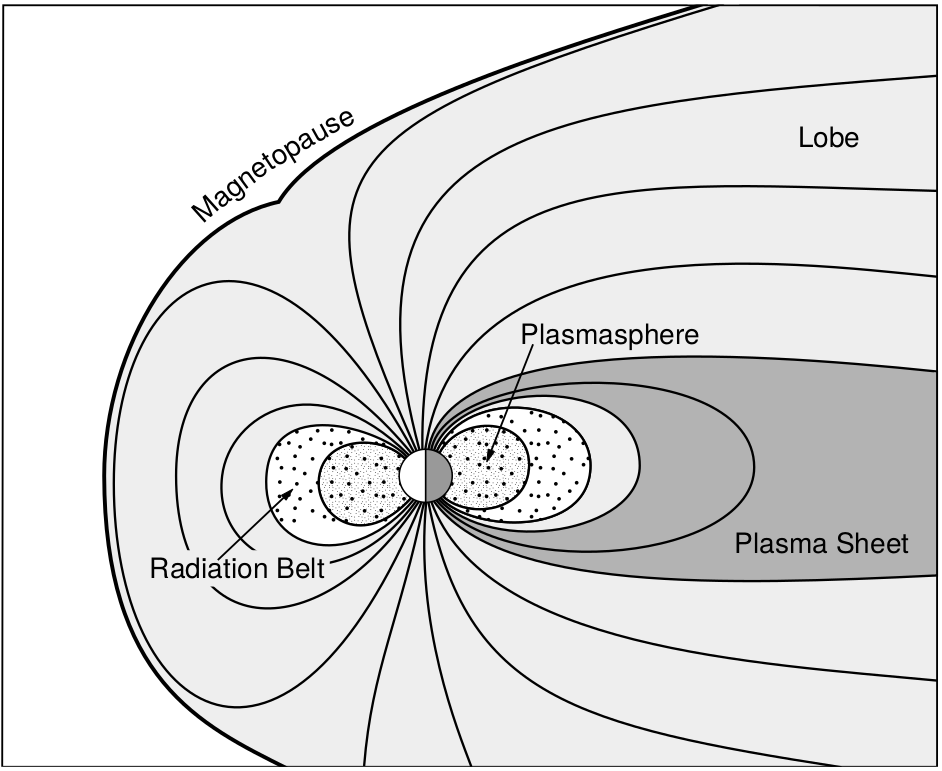
\includegraphics[width=\textwidth]{1_inner_magnetosphere.png}
\caption{A few macroscopic structures in the magnetosphere. The magnetosphere boundary with the solar wind is the magnetopause. The magnetotail consists of two lobes that contain Earth's magnetic flux with the plasma sheet separating the two lobes. The inner magnetosphere contains the plasmasphere, the ring current, and the radiation belts which are co-located. Figure from \citet{Baumjohann1997}.}
\label{Intro:inner_magnetosphere}
\end{figure}

The sun and its solar wind are ultimately the source of energy input into the magnetosphere. The solar wind at Earth's orbit is a plasma traveling at supersonic speeds with an embedded interplanetary magnetic field (IMF). When the solar wind encounters Earth's magnetic field, the plasma can not easily penetrate into the magnetosphere. The plasma can not easily penetrate into the magnetosphere because it is frozen-in on the magnetic field lines because plasma has a nearly infinite conductivity. Thus the plasma and its magnetic field drapes around the magnetosphere, forming a cavity in the solar wind that qualitatively has a shape similar to in Fig. \ref{Intro:inner_magnetosphere}. The solar wind is supersonic at 1 AU so a bow shock exists upstream of the magnetosphere which compresses and heats the solar wind. Downstream of the bow shock, the solar wind plasma flows around the magnetosphere inside the magnetosheath. The magnetopause is the surface where the solar wind ram and Earth's magnetic pressures balance. To first order, the magnetopause can be thought of as a boundary between the solar wind and Earth's magnetosphere. The shocked plasma then flows past the Earth where it shapes the magnetotail. In the magnetotail, the magnetopause exists where the solar wind magnetic pressure balances Earth's magnetic field pressure in the lobes. The magnetotail extends on the order of 100 $R_E$ downstream of Earth, and the tailward stretching of magnetic field lines creates a region where Earth's earthward and anti-earthward magnetic fields are in proximity. In this region, the curl of $\vec{B}$ is non-zero, thus by Ampere's law there must be a current (called the plasma sheet) near the magnetic equator \citep[e.g.][]{Eastwood2015}.

\subsection{Populations in the Inner Magnetosphere}\label{Intro:inner_mag}
Closer to Earth, where the magnetic field is largely dipolar, are three plasma populations that comprise the inner magnetosphere: the plasmasphere, the ring current, and the radiation belts which are shown in Fig. \ref{Intro:inner_magnetosphere}. Before we describe these three particle populations in detail, we will introduce the coordinate system that most naturally describes the inner magnetosphere environment, and the electric fields that mostly effect low energy particles.

This coordinate system is shown in Fig. \ref{Intro:dipole_coords} and it naturally describes particles in a dipole magnetic field geometry. In this coordinate system the ``radial" coordinate is the L shell. The $L$-shell ($L$) is the distance from the Earth's center to the location where a particular magnetic field line crosses the magnetic equator, in units of Earth radii, $R_e = 6,371$ km. The azimuthal coordinate is the magnetic local time (MLT). For an observer above Earth's north pole looking down, MLT is defined to be 0 (midnight) in the anti-sunward direction and increases in the counter-clockwise direction with 6 at dawn, 12 at noon (sunward direction), and 18 at dusk. The final coordinate is the magnetic latitude, $\lambda$, which is analogous to the latitude coordinate in the spherical coordinate system and is defined to be 0 at the magnetic equator. This coordinate system naturally describes the inner magnetosphere populations described below.

\begin{figure}
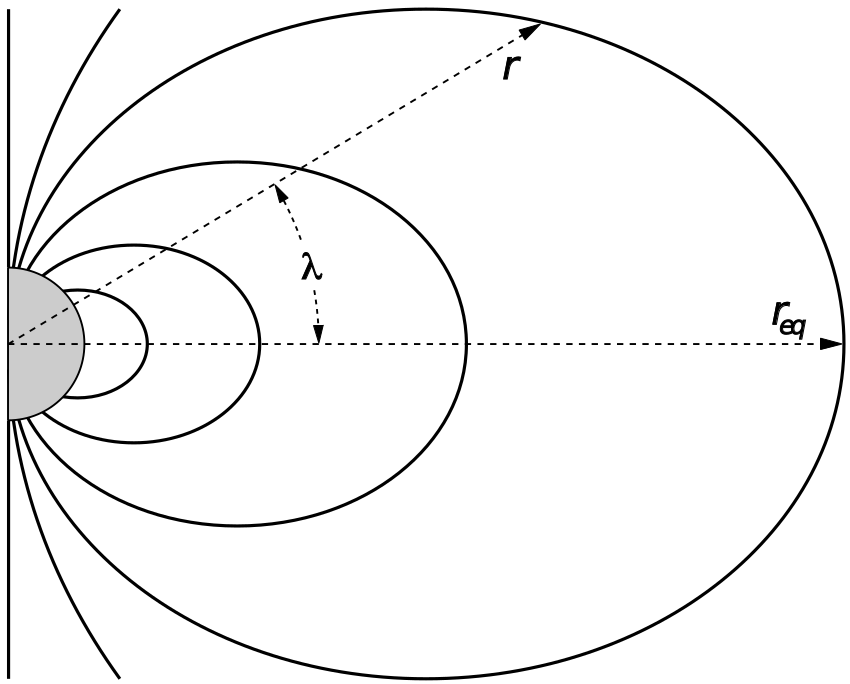
\includegraphics[width=\textwidth]{1_dipole_coords.png}
\caption{The dipole coordinate system. The magnetic latitude of $\mathbf{r}$ is $\lambda$. The radial distance to a magnetic field line in the equatorial plane is typically given by $L = r_{eq}/R_e$. Figure from \citet{Baumjohann1997}.}
\label{Intro:dipole_coords}
\end{figure}

Low energy particle dynamics in the inner magnetosphere are driven by the co-rotation and the dawn-dusk (pointing from approximately $6$ to $18$ MLT) electric fields. The co-rotation electric field arises from Earth's rotation. Earth's magnetic field and the particles frozen on it rotate with the Earth so in the magnetosphere (non-rotating) reference frame the particles appear to $\vec{E} \times \vec{B}$ drift (which will be described in the next section) with Earth's rotation. The co-rotation $\vec{E}$ points towards Earth. The convection electric field points from dawn to dusk, and is due to the Earthward transport of particles from the magnetotail. The superposition of the co-rotation and and convection electric fields is a potential field shown in Fig. \ref{Intro:E_fields}. The shaded area in Fig. \ref{Intro:E_fields} shows where low energy electrons execute closed orbits around Earth (i.e. particles are trapped), and outside this region the electrons are not trapped. The dynamic topology of the shaded region in Fig. \ref{Intro:E_fields} is controlled by only the convection electric field which is dependent on the solar wind speed and the IMF. The lowest energy particles that orbit along equipotential lines in the shaded region in Fig. \ref{Intro:E_fields} make up the plasmasphere.

\begin{figure}
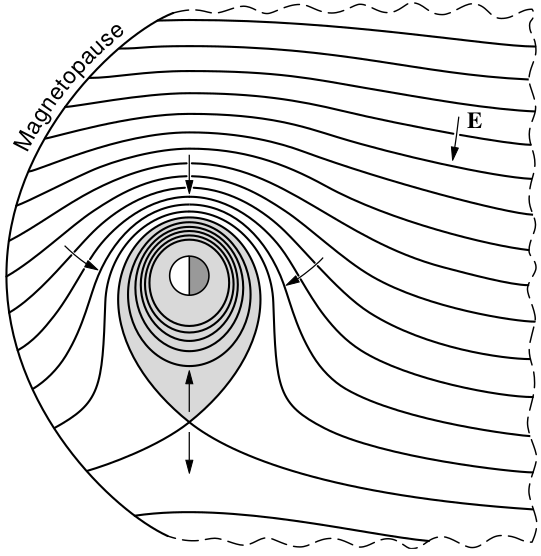
\includegraphics[width=\textwidth]{1_convection_corotation.png}
\caption{Equipotential lines and electric field arrows due to the superposition of the co-rotation and convection electric fields. Electrons in the shaded region execute closed orbits. Outside of the shaded regions the electrons are not trapped and will escape. The region separating the two regimes is called the Alfven layer. Figure from \citet{Baumjohann1997}.}
\label{Intro:E_fields}
\end{figure}

\subsubsection{Plasmasphere}
The plasmasphere is a relatively dense ($n_e \sim 10^3/\mathrm{cm}^3$) and cool ($\sim \mathrm{eV}$) plasma. The plasmasphere typically extends to $L \sim 4$ and the spatial extent is highly dependent on the solar wind and magnetospheric conditions. The source of the plasmasphere is the ionosphere, a layer in Earth's upper atmosphere that contains a high concentration of electrons and ions. The main mechanisms that ionize the ionosphere are ultraviolet light from the sun and particle precipitation. The ultraviolet ionization by sunlight is strongly dependent on the time of day and latitude, while particle precipitation is highly dependent on magnetospheric conditions and mostly occurs at high latitudes.

The outer boundary of the plasmasphere is called the plasmapause which is typically identified by a steep radial gradient in plasma density from $\sim 10^3 / \mathrm{cm}^3$ to $\sim 1 / \mathrm{cm}^3$. It is important to know the location of the plasmapause since the plasma density strongly controls the efficiency of particle scattering by waves. For example, electron scattering by chorus waves is more efficient when the ratio of the plasma and gyro frequency is low which is typically found in low plasma density regions outside of the plasmapause \citep[e.g.][]{Horne2003c, Horne2005, O'Brien2003empirical}.

\subsubsection{Ring Current}
A higher energy population is the ring current. This population consists of protons and electrons between tens and a few hundred keV that drift around the Earth. The orbits of higher energy particles are not as affected by the convection and co-rotation electric field, instead they drift around the Earth due to gradient and curvature drifts which will be described in the following section. Since the direction of the drift is dependent on charge, protons drift west around the Earth and electrons drift East. This effect creates a current around the Earth. 

The ring current generates a magnetic field which decreases the magnetic field strength at the surface of the Earth and increases it outside of the ring current. The decrease of Earth's magnetic field strength is readily observed by a system of ground-based magnetometers and is merged into a Disturbance Storm Time (DST) index to quantify the global reduction in the magnetic field. An example of a DST index time series from the 2015 St. Patrick's Day storm, driven by a coronal mass ejection (CME), is shown in Fig. \ref{Intro:dst}. At the start of a storm, DST sometimes increases in response to the compression of the magnetopause by a shock wave (termed the initial phase or sudden storm commencement) and is shown by the red horizontal bar in Fig. \ref{Intro:dst}. During the main phase of the storm the ring current population is rapidly built up and DST rapidly decreases which is shown by the green bar in Fig. \ref{Intro:dst}. After the storm is over, the ring current slowly recovers to pre-storm conditions during the recovery phase shown by the blue bar in Fig. \ref{Intro:dst}. In the recovery phase, the ring current gradually decays due to particles losses into the atmosphere, or transport through the magnetopause via mechanisms described later in this chapter. The DST index, along with other geomagnetic indicies, are used by the space physics community to quantify the global state of the magnetosphere.

\begin{figure}
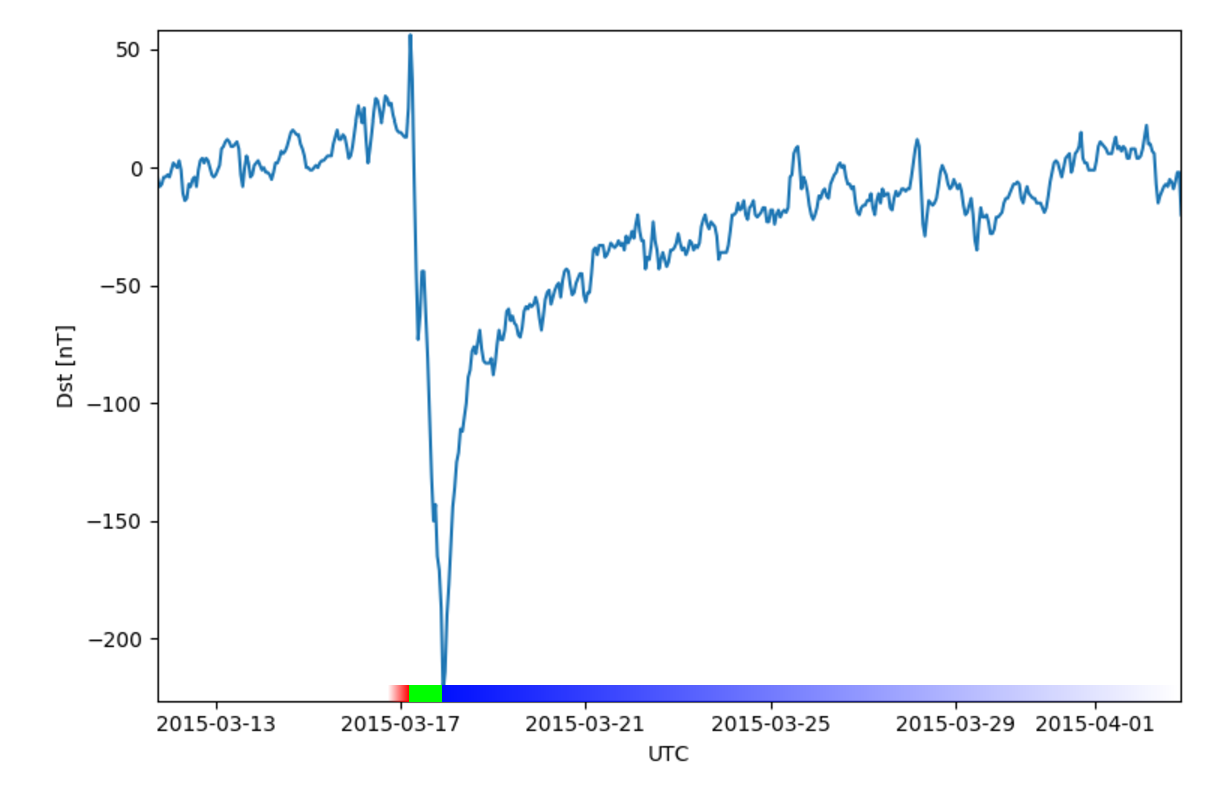
\includegraphics[width=\textwidth]{1_dst.pdf}
\caption{The DST index during the St. Patrick's Day 2015 storm. This storm was caused by a coronal mass ejection on March 15th, 2015. The storm phases are: initial phase, main phase, and recovery phase. The initial phase occurred when the Dst peaked at +50 nT on March 17th during which the ring current was eroded by the coronal mass ejection during the interval shown by the red bar shown at the bottom. Then the following rapid decrease to $\approx -200$ nT was during the main phase where many injections from the magnetotail enhanced the ring current, which reduced Earth's magnetic field strength at the ground, and is shown with the green bar. Lastly, the recovery phase lasted from March 18th to approximately March 29th during which the ring current particles were lost and the ring current returned to its equilibrium state. The recovery phase is shown with the blue bar.}
\label{Intro:dst}
\end{figure}

\subsubsection{Radiation Belts}\label{Intro:radiation_belt}
The highest particle energy populations are in the Van Allen radiation belts. These belts were discovered by \citet{Allen1959} and \citet{Vernov1960} during the Cold War and are a pair of toroidally shaped populations of trapped electrons and protons shown in Fig. \ref{Intro:rad_belts}. Their quiescent toroidal shape, similar to the shape of the plasmasphere and ring current, is a result of Earth's dipole magnetic field.

\begin{figure}
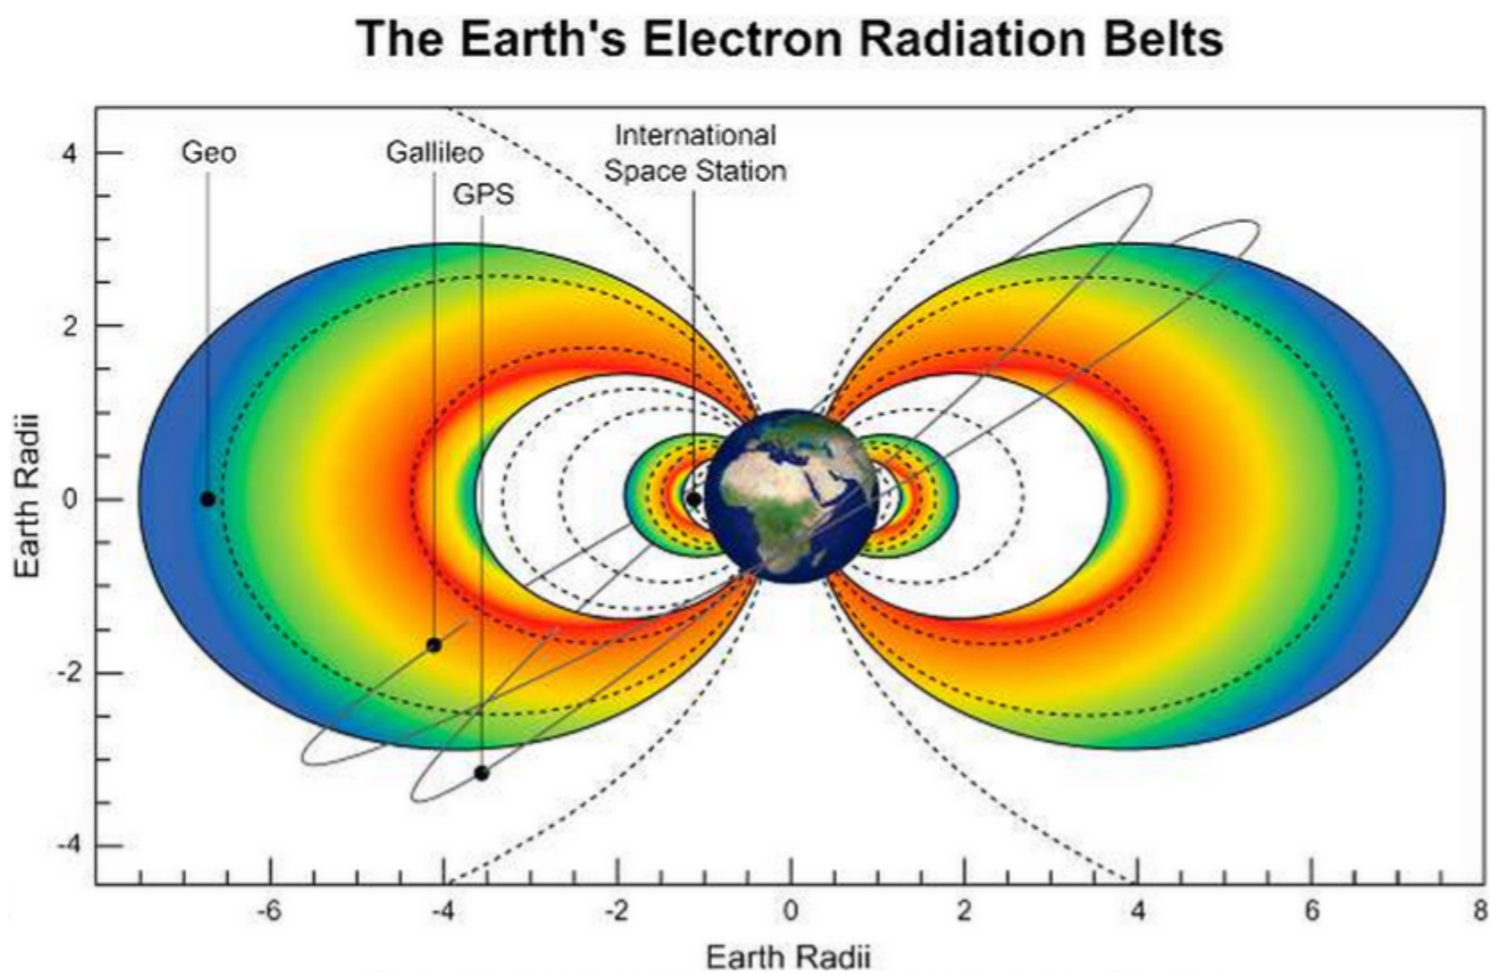
\includegraphics[width=\textwidth]{1_rad_belt.png}
\caption{The two radiation belts with a the locations of various satellites and orbits. Figure from \citep{Horne2013}.}
\label{Intro:rad_belts}
\end{figure}

\begin{figure}
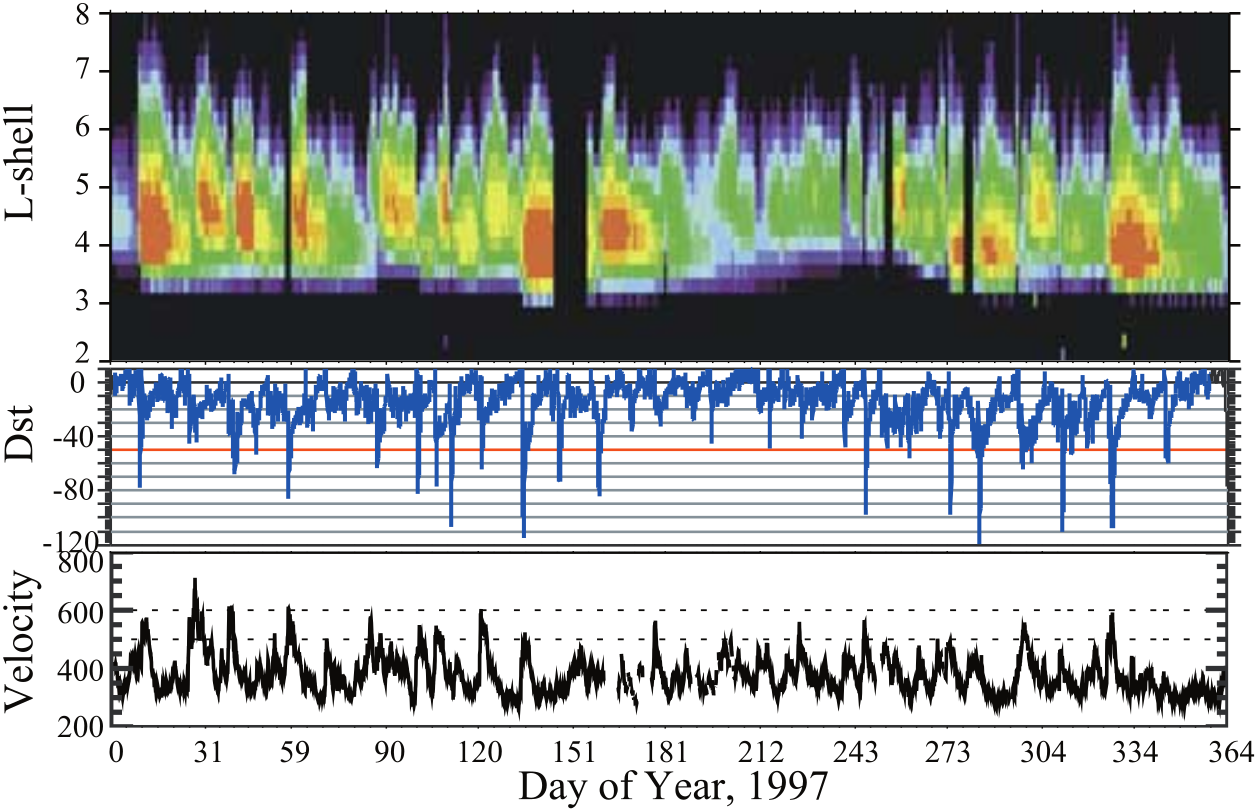
\includegraphics[width=\textwidth]{1_reeves_l_cut.png}
\caption{The dynamics of the outer radiation belt in 1997 from the POLAR satellite. Top panel shows the 1.2-2.4 MeV electron flux as a function of L and 1997 day of year. The middle panel shows the DST index, and bottom panel shows the solar wind velocity. Figure from \citep{Reeves2003}.}
\label{Intro:reeves_l_cut}
\end{figure}

The inner radiation belt is extremely stable on year time periods, extends to $L \approx 3$, and mainly consists of protons with energies between MeV and GeV and electrons with energies up to $\approx 1$ MeV \citep{Claudepierre2019}. The source of inner radiation belt protons is believed to be due to cosmic-ray albedo neutron decay \citep[e.g.][]{Li2017_CRAND} and inward radial diffusion for electrons \citep[e.g.][]{O'Brien2016_inner}. The gap between the inner and outer radiation belt is called the slot, which is believed to be due to hiss waves inside the plasmasphere (described below) scattering particles into the atmosphere \citep[e.g.][]{Lyons1973, Breneman2015}.

The outer radiation belt is much more dynamic and consists of mainly electrons of energies up to a few MeV. The outer belt's spatial extent is highly variable as shown in Fig. \ref{Intro:reeves_l_cut}, and is typically observed between L of $4$ and $8$. The source of outer radiation belt electrons is widely believed to be injections of plasma from the magnetotail that is then accelerated to high energies.

\section{Charged Particle Motion in Electric and Magnetic Fields}\label{Intro:particle_motion}
A charged particle trapped in the magnetosphere will experience three types of periodic motion in Earth's nearly dipolar magnetic field in the absence of electric fields. The three motions are ultimately due to the Lorentz force that a particle of momentum $\vec{p}$, charge $q$, and velocity $\vec{v}$ experiences in an electric field $\vec{E}$ and magnetic field $\vec{B}$ and is given by
\begin{equation} \label{Intro:Lorentz}
\frac{d\vec{p}}{dt} = q(\vec{E} + \vec{v} \times \vec{B}).
\end{equation} For many vector quantities in this dissertation, we will adopt a widely-used convention by splitting up vectors into parallel, $x_{||}$, and perpendicular, $x_\perp$ components with respect to the background magnetic field. In the magnetosphere, the three periodic motions, in decreasing frequency, are gyration, bounce, and drift and are schematically shown in Fig. \ref{Intro:motion_diagram}. Each periodic motion has a corresponding conserved quantity or adiabatic invariant. 

\begin{figure}
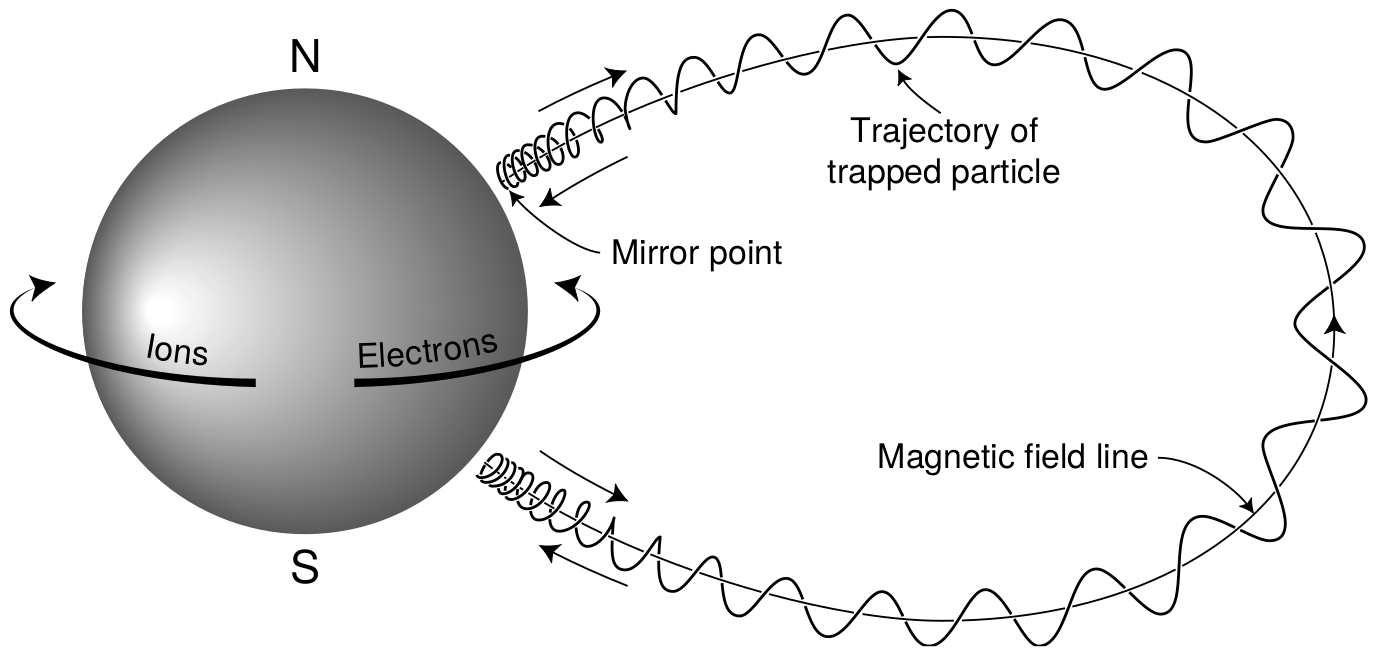
\includegraphics[width=\textwidth]{1_three_motions.png}
\caption{The three periodic motions of charged particles in Earth's dipole magnetic field. These motions are: gyration about the magnetic field line, bounce motion between the magnetic poles, and azimuthal drift around the Earth. Figure from \citep{Baumjohann1997}.}
\label{Intro:motion_diagram}
\end{figure}


The highest frequency periodic motion is gyration about a magnetic field of magnitude $B$. This motion is circular with a Larmor radius of 
\begin{equation}
r = \frac{m v_\perp}{|q| B}
\end{equation} where $m$ is the mass and $v_\perp$ the particle's velocity perpendicular to $\vec{B}$. This motion has a corresponding gyrofrequency of
\begin{equation}
\Omega = \frac{|q| B}{m}
\end{equation} in units of radians/second. In the radiation belts, the electron gyrofrequency, $\Omega_e$, is on the order of a kHz near the magnetic equator. The corresponding adiabatic invariant is found by integrating the particle's canonical momentum around the particle's path of gyration,
\begin{equation} \label{J}
J_i = \oint (\vec{p} + q \vec{A}) \cdot d\vec{l}
\end{equation} where $J_i$ is the $i^{th}$ adiabatic invariant and $\vec{A}$ is the magnetic vector potential. This integral is carried out by integrating the first term over the circumference of the gyro orbit and integrating the second term using Stokes theorem to calculate the magnetic flux enclosed by the gyro orbit.  The gyration invariant is $J_1 \sim v_\perp^2 / B$ which is conserved when the frequency, $\omega$, of a force acting on the gyrating electron satisfies $\omega << \Omega_e$.

The second highest frequency periodic motion is bouncing due to a parallel gradient in $\vec{B}$. This periodic motion naturally arises in the magnetosphere because Earth's magnetic field is stronger near the poles. To understand this motion we first we need to define the concept of pitch angle, $\alpha$ as the angle between $\vec{B}$ and $\vec{v}$ which is schematically shown in Fig. \ref{Intro:pa}a. The pitch angle relates $v$ with $v_\perp$ and $v_{||}$, the component of the particles velocity parallel to $\vec{B}$. As shown in Fig. \ref{Intro:pa}b and \ref{Intro:pa}c, a smaller (larger) $\alpha$ will increase (decrease) the distance that the charged particle travels parallel to $\vec{B}$ during one gyration.

Assuming the particle's kinetic energy is conserved, the conservation of $J_1$ implies that given a particle's $v_\perp(0)$ and $B(0)$ at the magnetic equator (where Earth's magnetic field is usually at a minimum) we can calculate its $v_\perp(s)$ along the particle's path, $s$, by calculating $B(s)$ from magnetic field models. Thus the particle's perpendicular velocity is then related via
\begin{equation} \label{j1_conservation}
\frac{v_\perp^2 (0)}{B(0)} = \frac{v_\perp^2 (s)}{B(s)}
\end{equation} which can be rewritten as 

\begin{equation}
\frac{v^2 \sin^2{\alpha(0)}}{B(0)} = \frac{v^2 - v^2_{||}(s)}{B(s)}
\end{equation} and re-arranged to solve for $v_{||}(s)$ by

\begin{equation} \label{Intro:eq_vp} 
v_{||}(s) = v \sqrt{1 - \frac{B(s)}{B(0)} \sin^2{\alpha(0)}}
\end{equation} which will tend towards 0 as the second term in the radical approaches 1.

The location where $v_{||}(s) = 0$ is called the mirror point and is where a particle stops and reverses direction. Since Earth's magnetic field is stronger towards both poles, the mirroring particle will execute periodic bounce motion between two mirror points in the northern and southern hemispheres. The corresponding adiabatic invariant, $J_2$ is

\begin{equation} \label{Intro:j2}
J_2 = \oint p_{||} ds
\end{equation} where $ds$ describes the particle path between the mirror points in the northern and southern hemispheres (see Fig. \ref{Intro:motion_diagram}). $J_2$ is found by substituting Eq. \ref{Intro:eq_vp} into Eq. \ref{Intro:j2} and defining the magnetic field strength at the mirror points as $B_m$ (where $\alpha(m) = 90^\circ$). The $J_2$ integral can be written as     
\begin{equation}
J_2 = 2 p \int_{m_n}^{m_s} \sqrt{1 - \frac{B(s)}{B(m)}} ds
\end{equation} where $m_n$ and $m_s$ are the northern and southern mirror points, respectively. The bounce period can be estimated \citep[e.g.][]{Baumjohann1997} to be 

\begin{equation}
t_b \approx \frac{L R_e}{\sqrt{W/m}} (3.7 - 1.6 \sin{\alpha(0)})
\end{equation} where $W$ is the particle's kinetic energy. As with gyration, the particle will bounce between the mirror points as long as $\omega << \Omega_b$, where $\Omega_b$ is the bounce frequency.

At this stage it is instructional to introduce loss cone pitch angle, $\alpha_L$.  Conventionally, the loss cone pitch angle is defined as the pitch angle where a particle will mirror at $\approx 100$ km altitude in the atmosphere. A charged particle gyrating at those altitudes will encounter, and likely Coulomb scatter, with the dense atmosphere and be lost. The $100$ km altitude is only a convention and not a hard boundary, e.g. the peak in the 1 MeV electron ionization rate is at $\approx 60$ km altitudes \citep{Fang2010}.

\begin{figure}
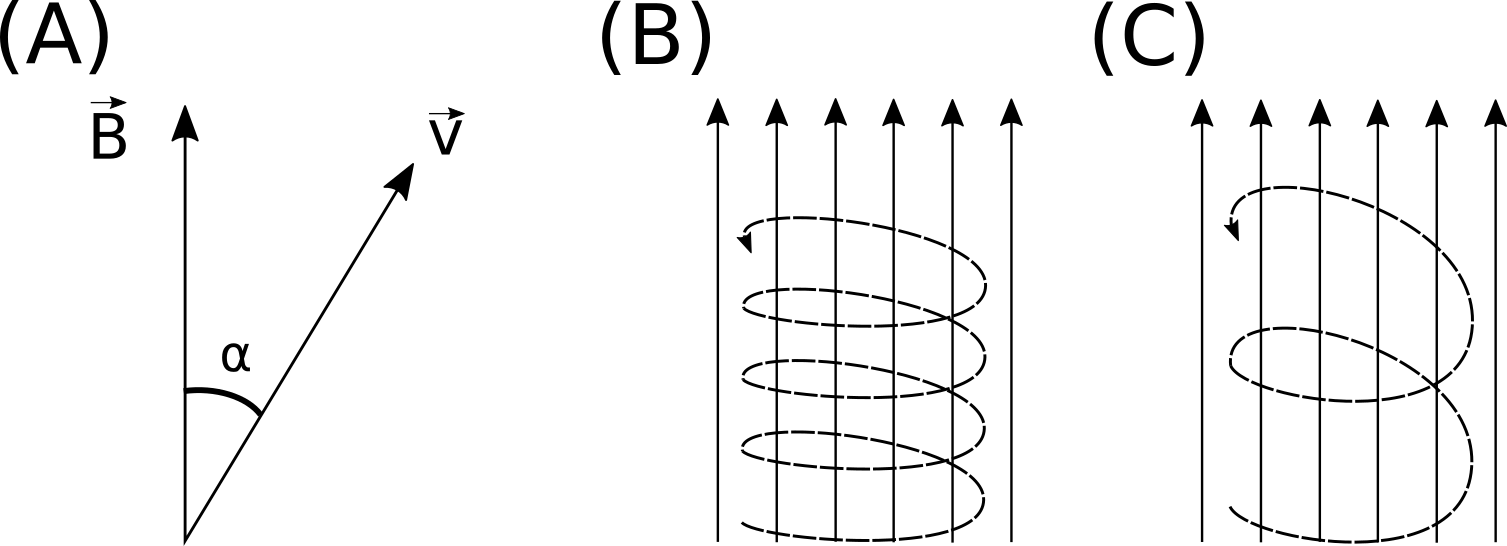
\includegraphics[scale=1]{1_pitch_angle_and_helix.png}
\caption{Charged particle motion in a uniform magnetic field $\vec{B}$. Panel (A) shows the geometry defining the pitch angle, $\alpha$. Panel (B) and (C) show two helical electron trajectories with dashed lines assuming a large and small $\alpha$ (corresponding to a small and large parallel velocity $v_{||}$), respectively.}
\label{Intro:pa}
\end{figure}

The slowest periodic motion experienced by charged particles in Earth's magnetic field is azimuthal drift around the Earth. This drift primarily results from a combination of a radial gradient in $\vec{B}$ and the curvature of the magnetic field. The radial gradient drift arises because Earth's magnetic field is stronger near the Earth. The particle's gyroradius shrinks as it gyrates towards Earth, and expands when it gyrates away from Earth. The overall effect is the particle gyro orbit does not close on itself causing eastward drift of negatively charged particles and westward drift of positively charged particles. The radial gradient drift is further enhanced by the centrifugal force that a particle experiences as it bounces along the curved field lines. The drift adiabatic invariant, $J_3$ is found by integrating Eq. \ref{J} over the complete particle orbit around the Earth. The shape of this drift orbit is known as a drift shell, and can be visualized by rotating the trapped particle trajectory in Fig. \ref{Intro:motion_diagram} around the axis that connects the poles. For $J_3$, the first term is negligible and the second term is the magnetic flux enclosed by the drift shell, $\Phi_m$  i.e. $J_3 \sim \Phi_m$.

To quantify the frequencies of the three periodic motions, Fig. \ref{Intro:adiabatic_frequencies} from \citet{Schulz1974} shows contours of the gyration, bounce, and drift frequencies for electrons and protons in Earth's dipole magnetic field. 

\begin{figure}
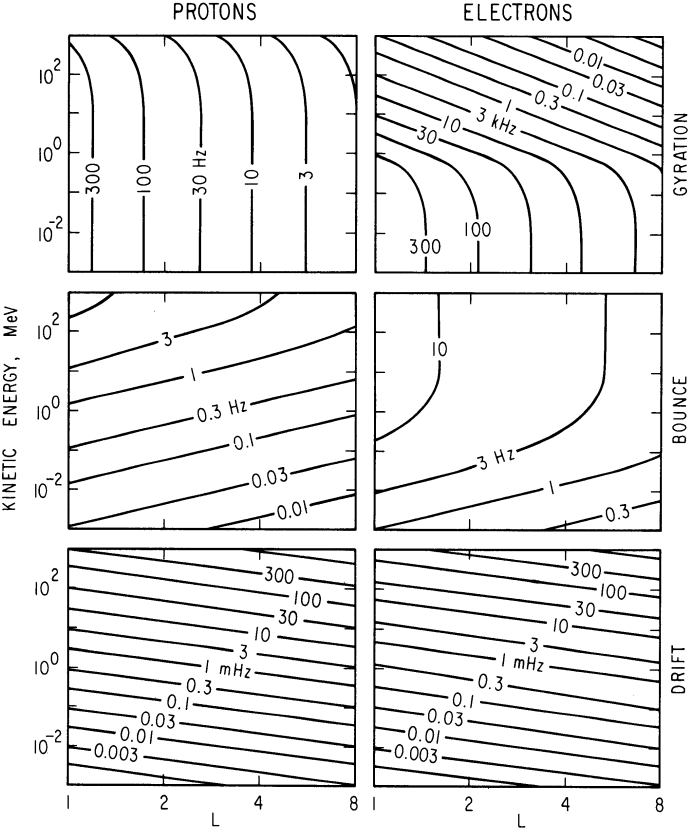
\includegraphics[width=\textwidth]{1_schulz_lanzerotti_fig6.png}
\caption{Contours of constant gyration, bounce, and drift frequencies for electrons and protons in a dipole field. Figure from \citet{Schulz1974}.}
\label{Intro:adiabatic_frequencies}
\end{figure}

Up until now we have considered the three periodic motions due Earth's magnetic field in the absence of electric fields. If there is an electric field, $\vec{E}$, perpendicular to $\vec{B}$, a particle's center of gyration (averaged position of the particle over a gyration) will drift with a velocity perpendicular to both $\vec{E}$ and $\vec{B}$. The drift velocity can be solved using Eq. \ref{Intro:Lorentz} and is
\begin{equation}
\vec{v}_E = \frac{\vec{E} \times \vec{B}}{B^2}.
\end{equation} If there is a parallel magnetic field, $E_{||}$, then the particle is accelerated along the magnetic field line. An $E_{||}$  pointing away from the Earth will contribute to the mirror force and raise the particle's mirror point. On the contrary, an Earthward pointing $E_{||}$ will oppose the mirror force and lower the mirror point. If the Earthward $E_{||}$ lowers the mirror point into the atmosphere, those particles will precipitate into the atmosphere. This is the mechanism that generates the aurora.

\section{Radiation Belt Particle Sources and Sinks}\label{Intro:sources_sinks}
Due to the highly energetic and dynamic nature of the radiation belts, and their impact on space exploration, the radiation belts have been studied for over half a century. Researchers have studied and attempted to predict the dynamics of radiation belt particles, waves, and wave-particle interactions by considering various competing particle acceleration and loss mechanisms which are described below.

%In the magnetosphere there are a variety of mechanisms that add and remove particles. In the radiation belts, there is a complex interplay between these mechanisms that cause substantial changes to the radiation belt particle fluxes. An example of the complex radiation belt dynamics from 1997 is shown in the top panel in Fig. \ref{Intro:reeves_l_cut}. This section will introduce a few mechanisms that contribute to the highly dynamic radiation belt fluxes including: adiabatic heating, wave-resonance heating, magnetopause shadowing, and wave-particle scattering.

\subsection{Adiabatic Heating}\label{Intro:adiabatic_heating}
One of the particle heating and transport mechanisms arises from the earthward convection of particles. As shown in Eq. \ref{j1_conservation}, the conservation of $J_1$ implies that the initial and final $v_\perp$ depends on the change in the magnetic field magnitude. As a particle convects earthward $B_f > B_i$ and thus $v_\perp$ must also increase. The dipole magnetic field magnitude falls off radially as $B \sim L^{-3}$, and the change in $v^2_{\perp}$ as the particle convects towards a stronger magnetic field is
\begin{equation}
\frac{v_{\perp \ f}^2}{v_{\perp \ i}^2} = \bigg( \frac{L_i}{L_f} \bigg)^3.
\end{equation} For a particle convecting earthward, if $J_2$ is conserved, its $v_{||}$ also increases because the distance between the particle's mirror points decreases. Calculating the increase in $v_{||}$ is somewhat difficult and is approximately

\begin{equation}
\frac{v_{|| \ f}^2}{v_{|| \ i}^2} = \bigg( \frac{L_i}{L_f} \bigg)^k
\end{equation} where $k$ ranges from $2$ for equatorial pitch angles, $\alpha_{eq} = 0^\circ$, to $2.5$ for $\alpha_{eq} = 90^\circ$ \citep{Baumjohann1997}. Since the rate of adiabatic heating is greater in the perpendicular direction than heating in the parallel direction, an initially isotropic particle distribution will become anisotropic during its convection. These isotropic particles can then become unstable to wave growth and generate waves in order to reach equilibrium.


\subsection{Wave Resonance Heating}\label{Intro:wave_heating}
Another mechanism that heats particles is caused by particles resonating with plasma waves. A few of the electromagnetic wave modes responsible for particle acceleration (and scattering) relevant to radiation belt dynamics are hiss, whistler mode chorus (chorus), and electromagnetic ion cyclotron (EMIC) waves. These waves are created by the loss cone instability that is driven by an anisotropy of electrons for chorus waves, and protons for EMIC waves. The level of anisotropy can be quantified by the ratio of the perpendicular to parallel particle temperatures $(T_\perp/T_{||})$. A particle distribution is unstable when $T_\perp/T_{||} > 1$. Since electrons gyrate in a right-handed sense, the chorus waves also tend to be right hand circularly polarized \citep{Tsurutani1997}. The same argument also applies to protons and left hand circularly polarized EMIC waves. 

These circularly polarized waves can resonate with electrons and/or protons when their relative motion results in a static $\vec{E}$ in the particle's reference frame. One example of a resonance between a right hand circularly polarized wave and an electron is shown in Fig. \ref{Intro:resonance_diagram}. The electron's $v_{||}$ and the wave's parallel wave vector, $k_{||}$, are in opposite directions such that the wave frequency, $\omega$, is Doppler shifted to an integer multiple of the $\Omega_e$ where the electron feels a static electric field and is accelerated or decelerated. Quantitatively, this resonance condition is easier to understand with the following toy model.

\begin{figure}
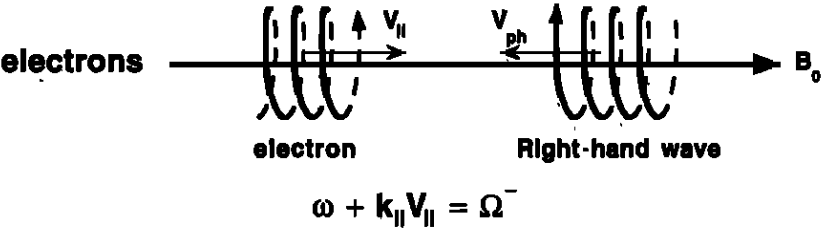
\includegraphics[width=\textwidth]{1_resonance.png}
\caption{The trajectories of an electron and a right-hand circularly polarized wave during a cyclotron resonance. The electron's $v_{||}$ and the wave's $k_{||}$ are in opposite directions such that the wave's frequency is Doppler shifted to a integer multiple of the electron cyclotron frequency. Figure from \citep{Tsurutani1997}.}
\label{Intro:resonance_diagram}
\end{figure}

Assume a uniform magnetic field, $\vec{B} = B_0 \hat{z}$, with a parallel propagating ($k = k\hat{z}$), right-hand circularly polarized wave. The wave's electric field as a function of position and time can be written as

\begin{equation}
\vec{E} = E_0 (\cos{(\omega t - kz)}\hat{x} + \sin{(\omega t - kz)}\hat{y}).
\end{equation} The angular component of $\vec{E}$ that will effect the particle's $v_\perp$ is 
\begin{equation}
E_\theta = \vec{E} \cdot \hat{\theta} = E_0 \cos{(\omega t - kz + \theta)}.
\end{equation} Now assume that the electron is traveling in the $-\hat{z}$ direction with a velocity, $\vec{v} = -v_0 \hat{z}$, so its time dependent position along $\hat{z}$ is

\begin{equation}
z(t) = -v_0 t
\end{equation} and gyrophase is

\begin{equation}
\theta(t) = -\Omega t + \theta(0)
\end{equation} where the first negative sign comes from the electron's negative charge. Now we put this all together into Eq. \ref{Intro:Lorentz} and find the force that the electron will experience

\begin{equation}
m \frac{dv_\theta}{dt} = qE_\theta = qE_0 \sin{((\omega + kv_0 - \Omega)t + \theta(0))}.
\end{equation} This is a relatively complex expression, but when the time dependent component is zero, i.e. 

\begin{equation} \label{Intro:resonance}
\omega + kv_0 - \Omega = 0,
\end{equation} the electron will feel a static electric field and be accelerated or decelerated depending on $\theta(0)$, the phase between the wave and the electron. The expression in Eq. \ref{Intro:resonance} is commonly referred to as the resonance condition and is more generally written as 

\begin{equation} \label{Intro:resonance_general}
\omega - k_{||} v_{||} = \frac{n \Omega_e}{\gamma}
\end{equation} where $n$ is the resonance order, and $\gamma$ is the relativistic correction \citep[e.g.][]{Millan2007}. In the case of the cyclotron resonance ($n = 1$), the wave and cyclotron frequencies are approximately equal and thus $J_1$ is violated. Since $J_1$ is violated, $J_2$ and $J_3$ are also violated since the conditions required to violate $J_2$ and $J_3$ are less stringent than $J_1$. 

It is important to remember that a particle will experience the effects of many waves along its drift orbit. The typical MLT extent of a handful of waves that are capable of resonating with radiation belt electrons are shown in Fig. \ref{Intro:waves}.

\begin{figure}
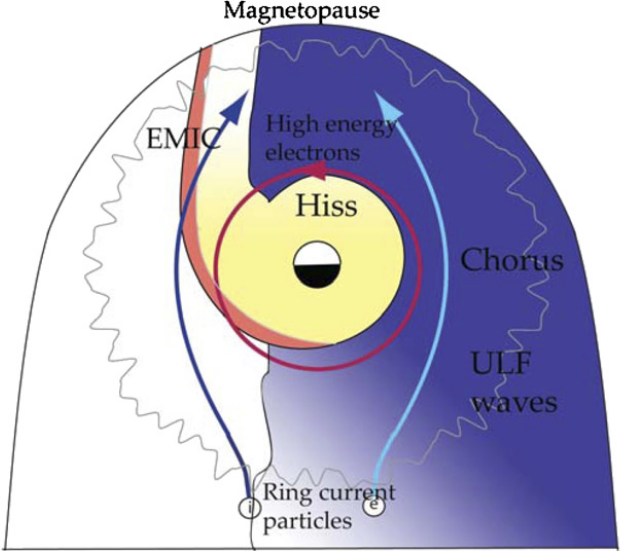
\includegraphics[width=\textwidth]{1_wave_populations.png}
\caption{Various wave modes in the magnetosphere. Ultra low frequency waves occur throught the magnetosphere. Chorus waves are typically observed in the 0-12 midnight-dawn region. EMIC waves are typically observed in the dusk MLT sector. Hiss waves are observed inside the plasmasphere. Figure from \citet{Millan2007}.}
\label{Intro:waves}
\end{figure}

\subsection{Particle Losses}\label{Intro:losses}
Now that we have seen two general mechanisms with which particles are accelerated in the magnetosphere, we will consider a few specific mechanisms that remove particles from the magnetosphere into the atmosphere or the solar wind. One mechanism that transports magnetosperic particles into the solar wind is magnetopause shadowing \citep[e.g.][]{Ukhorskiy2006}. Magnetopause shadowing occurs when the ring current is strengthened and Earth's magnetic field strength is increased outside of the ring current. If the ring current increases slowly enough (such that $J_3$ is conserved), a particle drift shell will move outward to conserve $J_3$. If the particle's drift shell expands past the magnetopause, the particle will be lost to the solar wind.

Another particle loss (and acceleration) mechanism is called radial diffusion and is driven by ultra low frequency (ULF) modulation of Earth's magnetic field. For example, if the solar wind compresses the magnetopause on time scales shorter than the drift period, particles will experience radial diffusion. If the transport is radially inward, particles will be accelerated. On the other hand, radially outward radial diffusion can transport particles through the magnetopause where they will be lost to the solar wind. \citet{Reeves2013} investigated the driver of particle acceleration during the October 2012 storm and observationally found that inward radial diffusion was not dominant, rather local acceleration via wave-resonance heating appeared to be the dominant acceleration mechanism.

The loss mechanism central to this dissertation is pitch angle and energy scattering of electrons by waves. Some of the waves that scatter electrons in energy and pitch angle in the inner magnetosphere are: plasmaspheric hiss \citep[e.g.][]{O'Brien2014, Breneman2015}, EMIC waves \citep[e.g.][]{Hendry2017, Capannolo2019energetic}, and chorus waves \citep[e.g.][]{Breneman2017, Kasahara2018, Ozaki2019}. These wave-particle interactions occur when the resonance condition in Eq. \ref{Intro:resonance_general} is satisfied and the particle's energy and $\alpha$ is modified by the wave. More details regarding the theory of pitch angle and energy diffusion is given in Chapter \ref{CH:mageis_microburst}. If the wave changes $\alpha$ towards zero and $\alpha < \alpha_{L}$, then the particle's mirror point dips below $100$ km altitude where the particle can be lost from the magnetosphere. One manifestation of pitch angle scattering of particles into the loss cone are microbursts, a sub-second duration impulse of electrons.

\section{Microbursts}\label{Intro:microbursts}
Microbursts were first seen with high altitude balloons which measured bremsstrahlung X-rays emitted by microburst electrons impacting the atmosphere by \citet{Anderson1964}. In the following years, numerous balloon flights expanded our knowledge of non-relativistic ($< 500$ keV) microbursts by quantifying the microburst spatial extent, temporal width, occurrence frequency, extent in L and MLT, and their source. It is worth noting that relativistic microbursts have not yet been observed by high altitude balloons. The microburst source was initially believed to be either a local plasma instability or a propagating disturbance in the magnetosphere \citep{Trefall1966, Brown1965_2, Barcus1966, Parks1967}. Soon after, both non-relativistic and relativistic microburst electrons were directly observed in LEO with spacecraft including the Solar Anomalous and Magnetospheric Particle Explorer (SAMPEX) \citep[e.g.][]{Blake1996, Blum2015, Lorentzen2001a, Lorentzen2001b, Nakamura1995, Nakamura2000, O'Brien2003, O'Brien2004, Greeley2019, Douma2017, Douma2019},  Montana State University's (MSU) Focused Investigation of Relativistic Electron Bursts: Intensity, Range, and Dynamics II (FIREBIRD-II) \citep{Spence2012, Klumpar2015, Crew2016, Anderson2017, Breneman2017}, and Science Technologies Satellite (STSAT-I) \citep[e.g.][]{Lee2005, Lee2012}. An example microburst time series is shown in Fig. \ref{Intro:microbursts} and was observed by the FIREBIRD-II CubeSats. The prominent features of the example microbursts in Fig. \ref{Intro:microbursts} are their sub-second duration, half order of magnitude increase in count rate above the falling background, and their 200-800 keV energy extent.

\begin{figure}
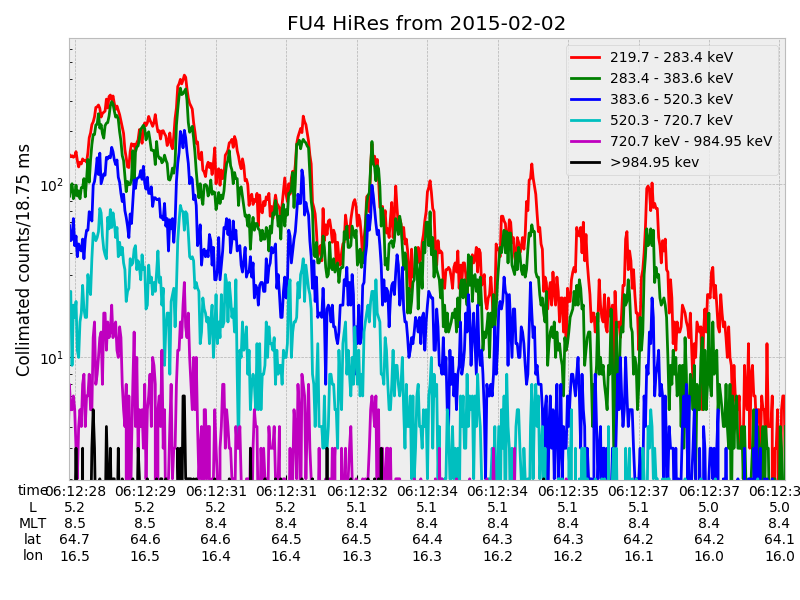
\includegraphics[width=\textwidth]{1_microbursts.png}
\caption{An example train of microbursts observed by FIREBIRD-II unit 4 on February 2nd, 2015. The colored curves show the differential energy channel count rates in five channels from $\approx 200$ keV to 1 MeV and a sixth integral energy channel with a 1 MeV threshold. The x-axis labels show auxiliary information such as time of observation and the spacecraft position in L, MLT, latitude and longitude coordinates.}
\label{Intro:microbursts}
\end{figure}

\begin{figure}
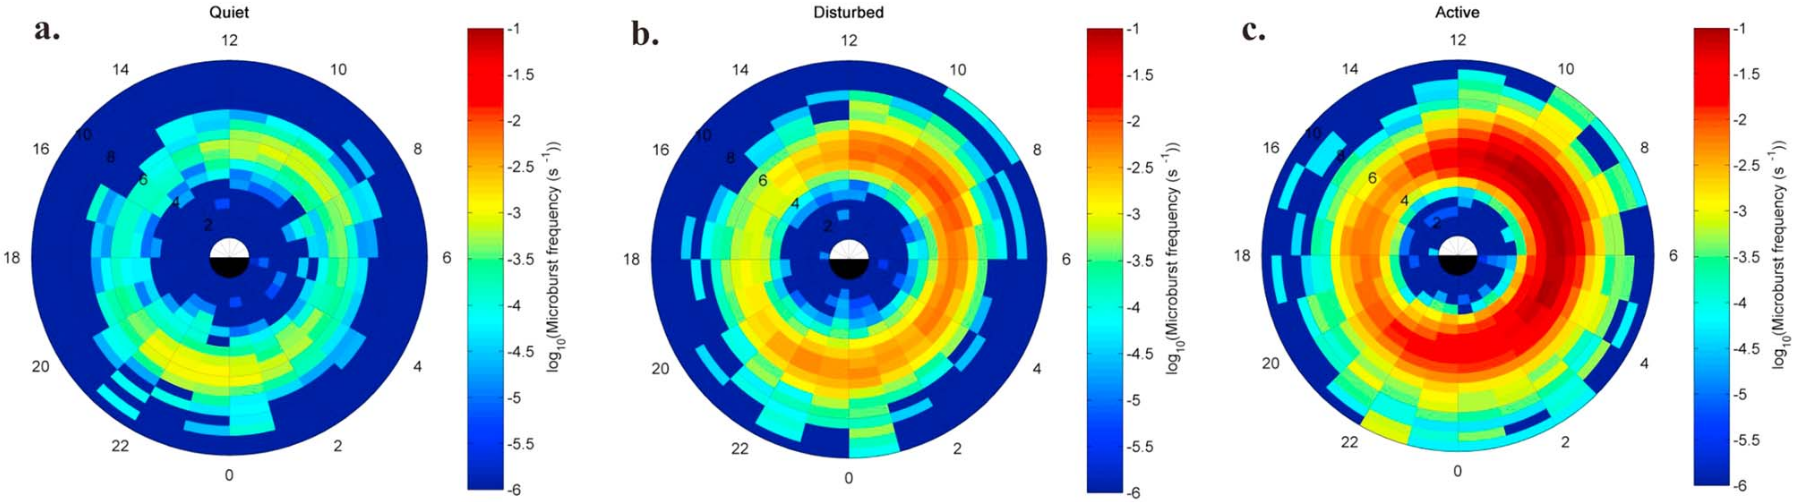
\includegraphics[width=\textwidth]{1_microburst_distribution_douma.png}
\caption{Distribution of $> 1$ MeV microburst occurrence rates as a function of L and MLT. The three panels show the microburst occurrence rate dependence on geomagnetic activity, parameterized by the auroral electrojet (AE) index for (a) $\mathrm{AE} < 100$ nT, (b) $100 < \mathrm{AE} < 300$ nT and (c) $\mathrm{AE} > 300$ nT. Figure from \citet{Douma2017}.}
\label{Intro:microburst_distribution}
\end{figure}

Microbursts are observed on magnetic field footprints that are connected to the outer radiation belt (approximately $4 < L < 8$). They are predominately observed in the 0-12 MLT sector with an elevated occurrence frequency during magnetospherically disturbed times as shown in Fig. \ref{Intro:microburst_distribution}. \citet{O'Brien2003} used SAMPEX relativistic electron data and found that microbursts predominately occur during the main phase of storms, with a heightened occurrence rate during the recovery phase. Microburst occurrence rates are also higher during high solar wind velocity events e.g. from co-rotating interaction regions \citep{O'Brien2003, Greeley2019}.

The estimated impact of microbursts on the atmosphere and the radiation belts is significant. Relativistic microburst electrons impacting the atmosphere are ionized at $<100$ km altitudes, with higher energy electrons penetrating closer to the surface. The resulting chemical reaction of microburst electrons impacting the atmosphere produces odd hydrogen $\mathrm{HO_x}$ and odd nitrogen $\mathrm{NO_x}$ molecules, which are partially responsible for destroying ozone ($\mathrm{O_3}$). \citet{Seppala2018} modeled a six hour relativistic microburst storm and found that the mesospheric ozone was reduced by $7-12 \%$ in the summer months and $12-20 \%$ in the winter months, so microbursts may have a non-negligible contribution to the dynamics of atmospheric ozone. Furthermore, microbursts have also been estimated to have a significant impact on the outer radiation belt electron population. The loss of all radiation belt electrons due to microbursts have been estimated to be on the order of a day \citep{Lorentzen2001b, O'Brien2004, Thorne2005, Breneman2017, Douma2019}. 

The wave-particle interactions responsible for generating microbursts are also believed to accelerate electrons in the radiation belts. As mentioned earlier, when an electron is in resonance with a wave, energy is exchanged with the wave and the electron is either accelerated or decelerated. The signature of wave-particle acceleration been observed for radiation belt electrons \citep[e.g.][]{Meredith2002, Horne2005, Reeves2013}, and \citet{O'Brien2003} presented evidence that enhancements in chorus waves, microbursts, and radiation belt electrons are related. To explain their observations, \citet{O'Brien2003} proposed that microburst precipitation is a side effect of electron acceleration due to chorus waves. 

The widely used theoretical framework to model the wave-particle interactions responsible for accelerating electrons and scattering microbursts is quasi-linear diffusion \citep[e.g.][]{Walker1993, Summers1998, Meredith2002, Horne2005, Thorne2005, Summers2005}. This framework is explained in Chapter \ref{CH:mageis_microburst}, and applied to an observation of a microburst in the heart of the radiation belt. Qualitatively, when a particle is resonant with a wave it can either be transported in pitch angle towards the loss cone and lose energy to the wave, or transported away from the loss cone and gain energy from the wave.

As previously mentioned, the range of observed microburst energies range from a few tens of keV \citep[e.g][]{Datta1997, Parks1967} to greater than 1 MeV \citep[e.g.][]{Blake1996, Greeley2019}. The microburst electron flux ($J$) falls off in energy, and the microburst energy spectra is typically well fit to a decaying exponential 

\begin{equation}
J(E) = J_0 e^{-E/E_0}
\end{equation} where $J_0$ is the flux at 0 keV (unphysical free parameter) and $E_0$ quantifies the efficiency of the scattering mechanism in energy \citep[e.g.][]{Parks1967, Datta1997, Lee2005}. A small $E_0$ suggests that mostly low energy particles are scattered. In contrast a high $E_0$ suggests that the scattering mechanism scatters low and high energy electrons. Reality is a bit more messy and a high $E_0$ may be a signature of a scattering mechanism that is most efficient at scattering high energy electrons, with a relatively minor efficiency to scatter low energy electrons. Since there are many more low energy electrons available to scatter, there may be relatively more low energy electrons scattered.

The short microburst duration, as observed by a single LEO satellite in a highly inclined orbit (motion is mostly latitudinal), has an ambiguity when interpreting what is a microburst. The two possible realities are: a microburst is very narrow in latitude and persistent, or transient. There are a few ways to distinguish between the two possible realities, and each one has a unique set of advantages.

A high altitude balloon essentially provides a stationary view of the precipitating particles under the radiation belt footprints. An intense transient microburst can be unambiguously identified above the slowly varying background. On the other hand, if the microburst precipitation is stationary, there will be too little contrast between the microburst and the background fluxes to be found.

Multi-spacecraft missions provide an alternate solution that can determine if a microburst is a spatial or a transient phenomena. As is illustrated in Fig. \ref{Intro:temporal_microburst}, a transient microburst can be recognized if two spacecraft, one trailing the other, simultaneously observe it. The size of the microburst footprint must then be larger than the spacecraft separation. On the contrary, if two spacecraft observe a microburst-like feature at the same location but at different times, then the feature is stationary and may be a curtain \citep{Blake2016}. Both balloon and multi-spacecraft observational methods have a unique set of strengths. This dissertation takes the multi-spacecraft approach to identify and study microbursts.

\begin{figure}
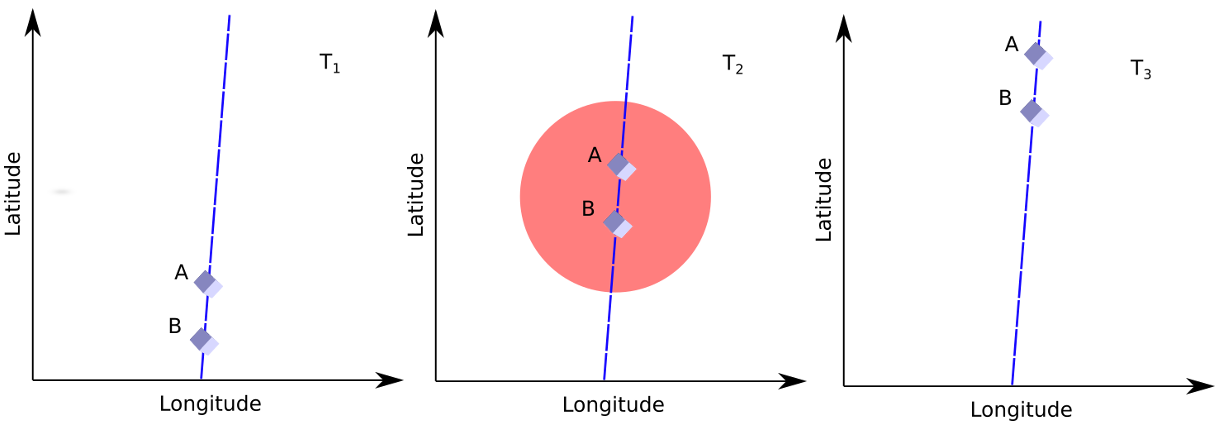
\includegraphics[width=\textwidth]{0_temporal_microburst.png}
\caption{Three snapshots of a temporal microburst observed simultaneously by a pair of polar-orbiting spacecraft. The spacecraft are identified by labels "A" and "B" and are traveling upwards on the blue dashed orbital track. At $T_1$ the spacecraft are traveling upwards and no microburst is observed. Then at $T_2$ both spacecraft simultaneously observe a microburst shown by the red circle and the microburst size must be greater than the spacecraft separation. In the last snapshot, $T_3$, the microburst has precipitated and no longer observed by the spacecraft.}
\label{Intro:temporal_microburst}
\end{figure}


\section{Scope of Reserach}\label{Intro:scope}
This dissertation furthers our understanding of the microburst scattering mechanism by presenting observational evidence of microburst scattering directly, and measuring microburst sizes and comparing them to the size of chorus waves. Chapter \ref{CH:mageis_microburst} describes a microburst scattering event observed by NASA's Van Allen Probes. For this event, particle and wave measurements were analyzed and modeled in the theoretical framework of pitch angle and energy diffusion. The following two chapters present studies of microburst sizes in comparison to chorus waves. Chapter \ref{CH:bouncing_packet} describes a bouncing packet microburst observation made by the FIREBIRD-II mission where the microburst's lower bound longitudinal and latitudinal sizes were estimated. Chapter \ref{CH:ac6_study} expands the case study from Chapter \ref{CH:bouncing_packet} to a statistical study of microburst sizes using The Aerospace Corporation's AeroCube-6 (AC6) CubeSats. In this study, a Monte Carlo and analytic microburst size models were developed to account for the compounding statistical effects of random microburst sizes and locations. Lastly, Chapter \ref{conclusions} will summarize this work and make concluding remarks regarding outstanding questions in microburst physics. % Change this to the tex file you want to compile.
%
%Contribution of Authors and Co-Authors Page
%\title{CHAPTER X \\ MICROBURST SCALE SIZE DERIVED FROM MULTIPLE BOUNCES OF A MICROBURST SIMULTANEOUSLY OBSERVED WITH THE FIREBIRD-II CUBESATS}

\chapter{MICROBURST SIZE DISTRIBUTION DERIVED WITH AEROCUBE-6} \label{CH:ac6_study}

\section{Contribution of Authors and Co-Authors} 
\noindent Manuscript in Chapter 1 \\ 

\noindent Author: M. Shumko \\
Contributions: Found microbursts in the AC6 data and calculated their size distribution.\\
Co-Author: A.T. Johnson \\
Contributions: Provided ideas and advice on how to analyze the AC6 data. \\
Co-Author: J.G. Sample \\
Contributions: Provided ideas and advice on how to analyze the AC6 data. \\
Co-Author: B.A. Griffith \\
Contributions: Checked the microburst detections by eye. \\
Co-Author: D.L. Turner \\
Contributions: Provided the initial inspiration for this project. \\
Co-Author: T.P. O’Brien \\
Contributions: Provided the initial inspiration for this project, proposed to use the cumulative distribution function analysis technique, and provided advise on how to use the AC6 data to address the noise issues.\\
Co-Author: O. Agapitov \\
Contributions: Provided the THEMIS wave dataset for the direct comparison of the microburst and chorus size distributions\\
Co-Author: J.B. Blake \\
Contributions: Provided advise on how to use the AC6 data and address the noise issues. \\
Co-Author: S. G. Claudepierre \\
Contributions: Checked the microburst size models and provided analysis advice \\
\newpage

\section{Manuscript Information}

\noindent M. Shumko, A.T. Johnson, J.G. Sample, B.A. Griffith, D.L. Turner, T.P. O’Brien, O. Agapitov, J.B. Blake, S. G. Claudepierre\\
Journal of Geophysical Research \\
Status of Manuscript: \textcolor{red}{Officially submitted to a peer-reviewed journal} \\
Wiley \\

\newpage

\section{Key Points}
\begin{itemize}
\item The dual AeroCube-6 CubeSats simultaneously observed $> 35$ keV microbursts at a variety of spatial separations ranging from $2$ to $\approx 100$ km.
\item In low Earth orbit the majority of microbursts have a size on the order of a few tens of km.
\item At the magnetic equator, the size of most microbursts corresponds to the size of whistler-mode chorus wave packets.
\end{itemize}

\section{Abstract}
Microbursts are an impulsive increase of electrons from the radiation belts into the atmosphere and have been directly observed in low Earth orbit and the upper atmosphere. Prior work has estimated that microbursts are capable of rapidly depleting the radiation belt electrons on the order of a day, hence their role to radiation belt electron losses must be considered. Losses due to microbursts are not well constrained, and more work is necessary to accurately quantify their contribution as a loss process. To address this question we present a statistical study of $> 35$ keV microburst sizes using the pair of AeroCube-6 CubeSats. The microburst size distribution in low Earth orbit and the magnetic equator was derived using both spacecraft. In low Earth orbit, the majority of microbursts were observed while the AeroCube-6 separation was less than a few tens of km, mostly in latitude. To account for the statistical effects of random microburst locations and sizes, a Monte Carlo and analytic models were developed to test hypothesized microburst size distributions. A family of microburst size distributions were tested and a Markov Chain Monte Carlo sampler was used to estimate the optimal distribution of the microburst size model parameters. Finally, a majority of observed microbursts map to sizes less then $200$ km at the magnetic equator. Since microburst are widely believed to be generated by scattering of radiation belt electrons by whistler mode waves, the observed microburst size correlates to coherent whistler mode chorus sizes derived in prior literature.

\section{Introduction}
Since the discovery of the Van Allen radiation belts in the 1960s by \citet{Allen1959} and \citet{Vernov1960}, decades of research has made headway in understanding the various particle acceleration and loss mechanisms. One of the extensively studied mechanisms responsible for both acceleration and loss is wave-particle scattering between whistler-mode chorus waves and electrons \citep{Abel1998_1, Meredith2002, Horne2003, Thorne2005, Millan2007, Bortnik2008}. Whistler-mode chorus waves are typically generated by a temperature anisotropy of low energy electrons up to tens of kiloelectronvolts (keV) and are typically found in the $\sim 0-12$ magnetic local times (MLT) \citep{Li2009, Li2009b}. Whistler-mode chorus waves interact with radiation belt electrons, and are widely believed to cause electron precipitation termed microbursts \citep[e.g.][]{Millan2007}.

Microbursts are a subsecond impulse of electrons that are observed by high altitude balloons and satellites in low Earth orbit (LEO) on radiation belt magnetic footprints $\sim 4 - 8$ L-shell (L) \citep[e.g.][]{Anderson1964, Lorentzen2001a, O'Brien2003, Tsurutani2013, Woodger2015, Crew2016, Breneman2017, Mozer2018, Greeley2019}, mostly in the dawn MLTs, and with an enhanced occurance rate during disturbed magnetospheric times \citep{O'Brien2003, Douma2017}. Microburst's role as a radiation belt electron loss mechanism has been estimated to be significant, with total radiation belt electron depletion due to microbursts estimated to be on the order of a day \citep{Lorentzen2001b, O'Brien2004, Thorne2005, Breneman2017}. These average microburst loss estimates are not well constrained due to assumptions made regarding the microburst precipitation region.

One of the unconstrained microburst parameters that is critical to better quantify the role of microbursts as an instantaneous loss mechanism (the number of electrons lost per microburst) is their physical size. Historically, after the bremsstrahlung X-ray signatures of microbursts were discovered by \citet{Anderson1964}, numerous microburst size studies were done using other balloon flights in the mid 1960s. \citet{Brown1965_2} used data from a pair of balloons separated by 150 km, mainly in longitude, and found that one third of all microbursts observed were temporally coincident. \citet{Trefall1966} then used the results from \citet{Brown1965_2} to model the probability that a microburst will be observed by two balloons as a function of the radius of the microburst, radius of the precipitating area a balloon is sensitive to, and the balloon separation. \citet{Trefall1966} concluded that the microbursts reported by  \citet{Brown1965_2} must have had a diameter of $230$ km assuming a balloon has a circular field of view with a $140$ km diameter (for electrons stopped at $100$ km altitudes). Soon after, \citet{Barcus1966} used a pair of balloons and concluded that a microburst must have a $<200$ km longitudinal extent. Then \citet{Parks1967} used data from a single balloon with four collimated scintillators oriented in different directions and found that the size of some mostly low energy microbursts to have a diameter of $80 \pm 28$ km, and others were less than $40$ km. 

Direct observations of microburst electrons are made by LEO spacecraft. \citet{Blake1996} found a microburst with a size of a few tens of km using the the Solar Anomalous and Magnetospheric Particle Explorer (SAMPEX) and concluded that typically microbursts are less than a few tens of electron gyroradii in size (order of a few km in LEO). Recently, \citet{Dietrich2010} used SAMPEX observations in another case study and concluded that the observed microbursts were smaller than $4$ km. \citet{Crew2016} used the Focused Investigation of Relativistic Electron Bursts: Intensity, Range, and Dynamics (FIREBIRD-II) CubeSats and found an example of a microburst larger than 11 km. Lastly, \citet{Shumko2018a} also used FIREBIRD-II to identify a microburst with a size greater than $ 51 \pm 1$ km. If anything, the large variance in prior results imply that there is a distribution of microburst scale sizes which this study aims to estimate.

Besides addressing the instantaneous radiation belt electron losses due to individual microbursts, the microburst size distribution is useful to identify the wave mode(s) responsible for scattering microbursts. By mapping the microburst size distribution in LEO to the magnetic equator it can be compared to the wave sizes estimated in prior literature. This comparison can be used to identify the waves and their properties (e.g. amplitude or coherence) responsible for scattering microburst electrons.

This paper addresses these two questions by expanding the prior microburst size case studies by analyzing microburst observations over a three year time period to estimate the microburst size distribution in LEO and the magnetic equator. The twin AeroCube-6 (AC6) CubeSats are utilized for this study because they were ideally equipped to observe microbursts simultaneously over a span of three years while their total separation varied between 2 and 800 km, mostly in latitude (in-track in orbit). This paper first describes the AC-6 mission, including their orbit and instrumentation in section \ref{instrumentation}. Section \ref{microburst_detection} develops the methodology used to identify microbursts observed by each spacecraft and how they were combined to make a list of simultaneously observed microbursts. Section \ref{microburst_distribution} describes the methodology used to estimate the microburst size distributions in LEO and the magnetic equator as a function of AC6 separation. Then a model is developed to shed light on how the compounding effects of a hypothesized microburst shape, size distribution, and random microburst locations will be observed by AC6, a two-point measurement platform. Lastly, in section \ref{discussion} we discuss these results and compare the microburst sizes estimated here to the size distribution of the whistler-mode chorus waves that are believed to cause microbursts. 

\section{Instrumentation} \label{instrumentation}
The AC6 mission consists of a pair of 0.5U (10x10x5 cm) CubeSats built by The Aerospace Corporation and launched on June 19th, 2014 into a 620 x 700 km, $98^\circ$ inclination orbit. The two satellites, designated as AC6-A and AC6-B, separated after launch and drifted apart. Both AC6 units have an active attitude control system which allows them to adjust the atmospheric drag experienced by each AC6 unit by orienting their solar panel ``wings" with respect to the ram direction. By changing their orientation, AC6 was able to achieve fine separation control and maintain a separation between 2-800 km. Figure \ref{fig1}a shows the AC6 separation for the duration of the mission. Figure \ref{fig1}b shows where AC6 was taking 10 Hz data simultaneously as a function of L and MLT which highlights that most data was taken at 8-12 MLT, an ideal local time for observing microbursts. Lastly Fig. \ref{fig1}b shows that the AC6 orbit was roughly dawn-dusk, sun-synchronous and precessed only a few hours in MLT over a three year period.

Each AC6 unit is equipped with three Aerospace microdosimeters (licensed to Teledyne Microelectronics, Inc). The dosimeter used for this study is dos1 and is identical on both AC6 units. Dos1 has a 35 keV electron threshold and all dosimeters sample at 1 Hz in survey mode, and 10 Hz in burst mode in the radiation belts. More detailed technical information on AC6 is described in \citet{O'brien2016}. 

\begin{figure}
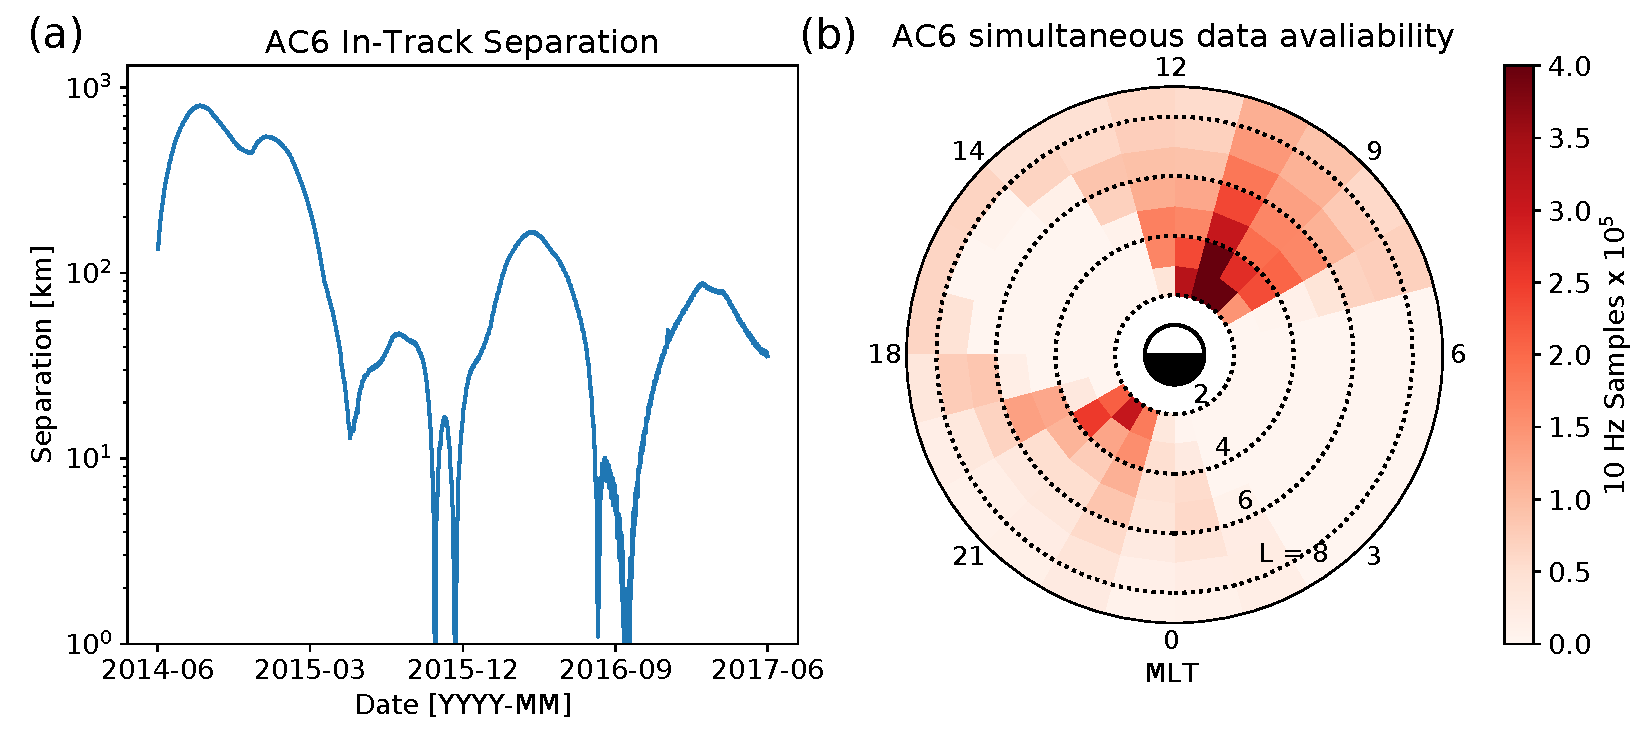
\includegraphics[width=\textwidth]{4_fig1.pdf}
\caption{AC6 mission properties for (a) spacecraft separation and (b) number of simultaneous quality 10 Hz samples as a function of L and MLT.} \label{fig1}
\end{figure}

\section{Methodology} 
\subsection{Microburst Detection} \label{microburst_detection}
The first step to find microbursts observed simultaneously by AC6 is to identify them on each individual spacecraft. Microbursts were detected with two different methods that yielded quantitatively similar results. The first method is the burst parameter \citep{O'Brien2003}. This algorithm has been successfully used in other microburst studies, mainly with the microbursts observed by SAMPEX \citep[e.g.][]{O'Brien2003, Blum2015, Douma2017}. For AC6, a burst parameter threshold of 5 was determined to be a good trade-off between false positive and false negative microburst detections. Another microburst detection algorithm based on wavelet spectra frequency filtering was developed and the resulting list of microbursts is similar to the list from the burst parameter.

With the two microburst detection lists in hand, data cleaning to remove microburst-like transmitter noise was necessary. The transmitters on AC6 can cause unphysical count impulses in the dosimeters that resembles periodic trains of microbursts. One source of transmitter noise was observed at times when AC6 was in contact with the ground stations above the US for data downloads and commanding, thus the microburst detections made above the US that were mostly at low L were discarded. 

Another source of noise is crosslink transmissions between AC6-A and AC6-B. These transmissions occurred when either spacecraft transitioned from the survey mode to 10 Hz mode. This noise is sometimes not caught by the data quality flag, so the following empirically-derived criteria were developed to remove those detections. The dosimeter with a 250 keV nominal electron threshold, dos2, was used because it had a nearly identical response to noise while rarely responded to microbursts. Since the transmitter noise is very periodic with a $\approx 0.2$ s period, cross-correlation (CC) and autocorrelation (AC) methods were applied to the dos1 and dos2 time series. Detections were discarded if the following two criteria were met: either dos1 or dos2 time series had a AC peak at a $0.2$ or $0.4$ s lag and the dos1-dos2 CC was greater than 0.9. The AC lag criteria alone sometimes falsely removed legitimate trains of microbursts, so the second criteria insured that the detection was removed if there was also an unphysically high correlation across an order of magnitude in energy.

The lists of microbursts observed individually by AC6 were then merged into a list of temporally correlated microbursts, i.e. microbursts that were observed simultaneously by both AC6 units, with the following procedure. The general idea is that a microburst detected by one spacecraft will cross-correlate well with the time series from the other spacecraft if it observed a similar microburst, and poorly if there was no microburst observed by the other spacecraft. Each microburst detection made by either spacecraft was cross-correlated with the time series from the other spacecraft whether or not a microburst was observed by the other spacecraft. Cross-correlation windows with 1 and 1.2 s widths were chosen with slightly different window sizes to account for random count variation due to Poisson noise. Microbursts detections that had a cross-correlation greater than $0.8$ were considered temporally coincident. This CC threshold was chosen as it is low enough to accept user-identified temporally coincident microbursts superposed with noise, and high enough to reject most non-coincident events. Figure \ref{fig2}, panels (a), (c), (e), and (g) show examples of microbursts observed by both AC6 units when they were separated by 5, 16, 37, and 69 km, respectively. 

The last criteria requires that the temporal CC must be greater than the spatial CC + 0.3. The spatial CC was calculated by shifting one spacecraft's time series by the in-track lag to cross-correlate in the same spatial location, i.e. latitude. This criteria was applied to remove curtains, stationary structures observed by AC6 that are narrow in latitude \citep{Blake2016} that can be misidentified as microbursts. Figure \ref{fig2}, panels (b), (d), (f), and (h) show the shifted time series to confirm that there were no spatially correlated, non-microburst structures present. Lastly the merged microburst list was spot checked by two authors to remove poorly correlated and any duplicate events. After filtering out transmitter noise and applying the CC criteria, 662 simultaneous microburst detections were found and used in this study.

\begin{figure}
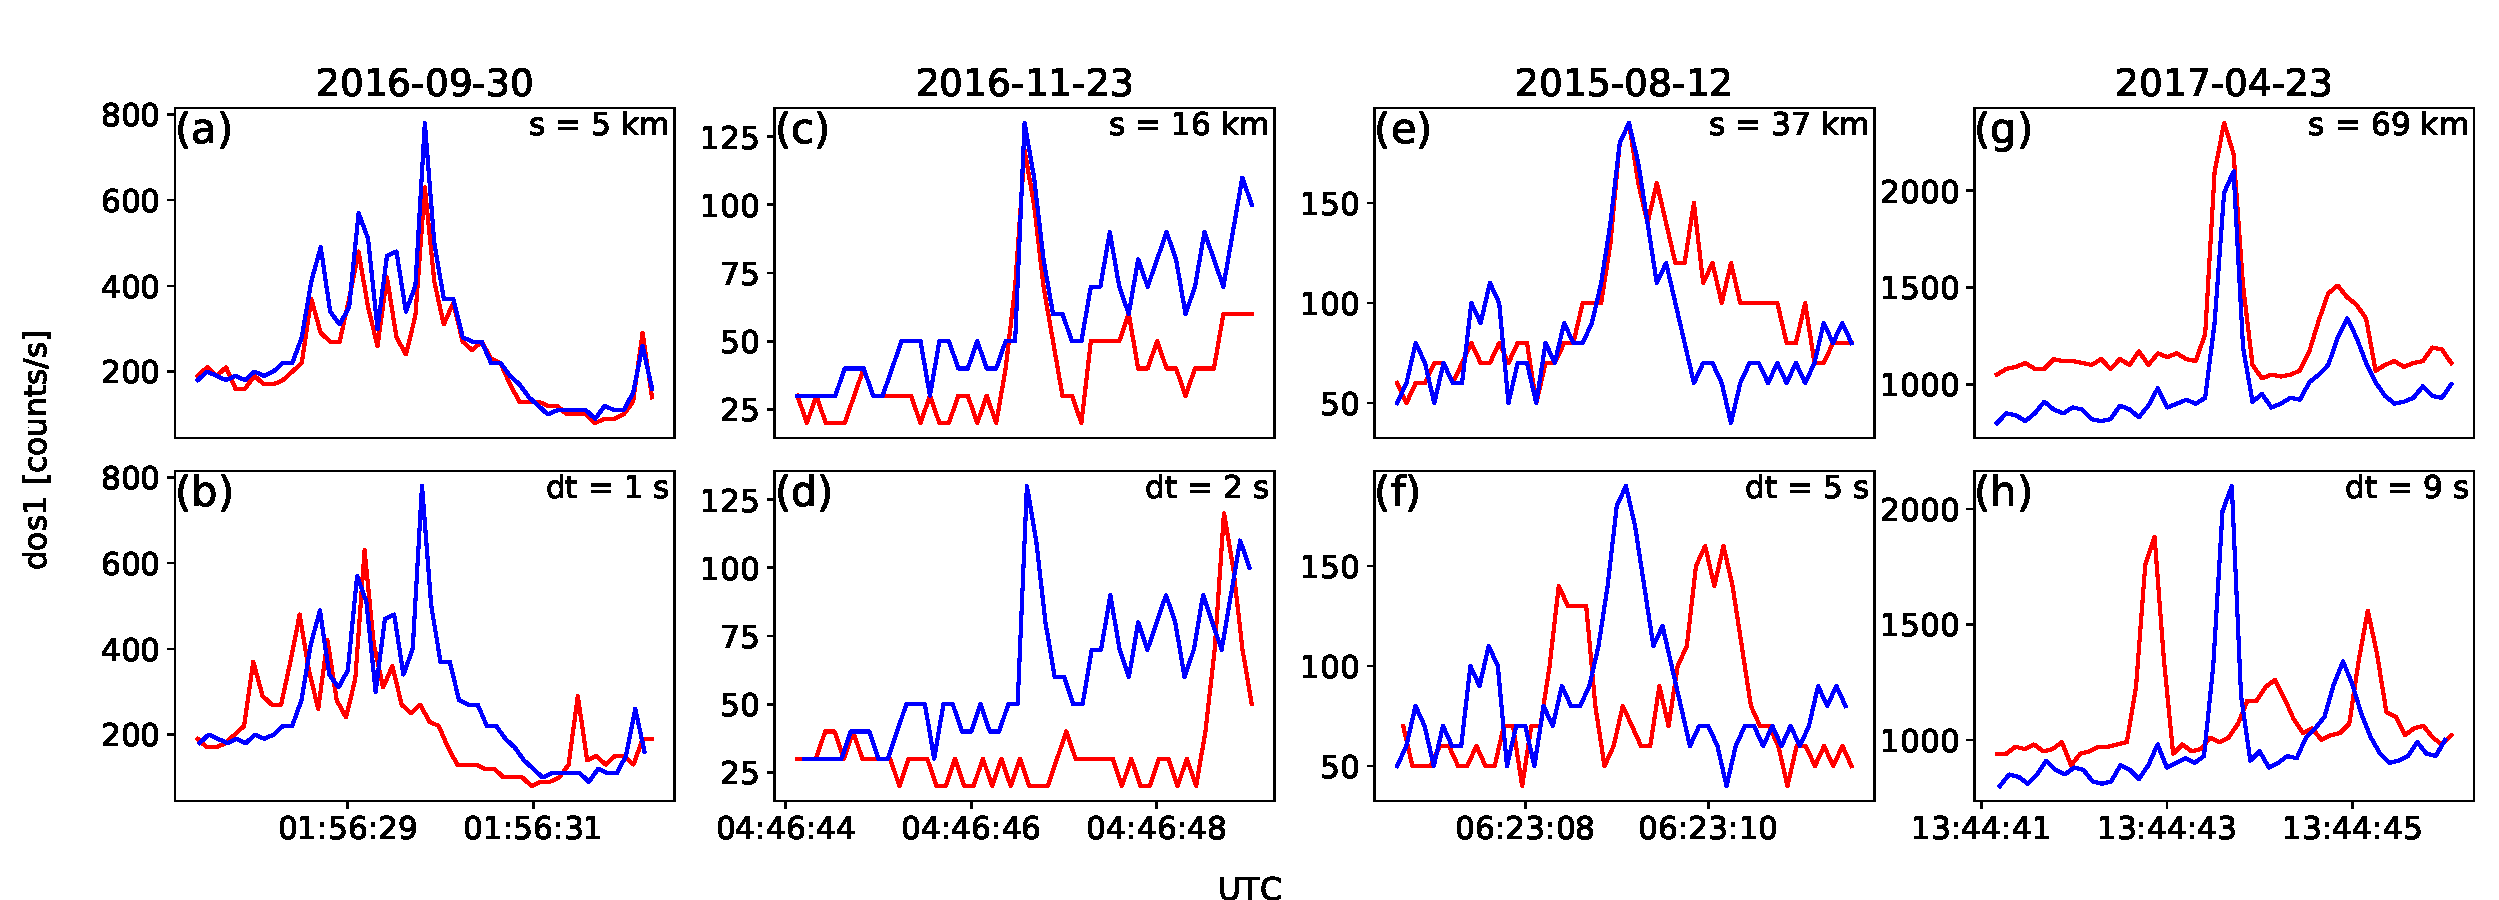
\includegraphics[width=\textwidth]{4_fig2.pdf}
\caption{Examples of $>35$ keV microbursts observed simultaneously by AC6-A in red and AC6-B in blue. Panels (a), (c), (e), and (g) show the temporally-aligned time series when AC6 were separated by $s=$ 5, 16, 37, and 69 km, respectively. The corresponding panels (b), (d), (f), and (h) show the spatially-aligned time series which is made by shifting the AC6-A time series in the above panels by the in-track lag (annotated with $dt$) that show any spatially correlated structures. The clear temporal correlation and lack of spatial correlation demonstrates that these events are microbursts.} 
\label{fig2}
\end{figure}
	

\subsection{Microburst Size Distribution in LEO and Magnetic Equator}\label{microburst_distribution}
The temporally coincident microbursts, which from now on will be referred to as microbursts, are now used to estimate the fraction of microbursts observed above AC6 separation, $s$. When AC6 observes a microburst at $s$, the microburst's size must be greater than $s$. This fact, along with the arguments presented in Section 4 in \citet{Joy2002} who studied the most probable Jovian magnetopause and bow shock stand off distances, are used to investigate the dependence of the number of microbursts observed above $s$, as a function of $s$. This dependence is the microburst complementary cumulative distribution function $\bar{F}(s)$. 

The cumulative fraction of microbursts observed above $s$ is the ratio of $N(s)$, the normalized number of microbursts observed above $s$, to $N(0)$, the total number of microbursts observed 
\begin{equation}
\bar{F}(s) = \frac{N(s)}{N(0)}
\end{equation} where N(s) is defined by

\begin{equation}
N(s) = \sum_{i = s}^\infty n_{i} \Big( \frac{S_{max}}{S_{i}} \Big)
\end{equation} where $n_{i}$ is the number of microbursts observed by AC6 in ith separation bin. The normalization term $S_{max}/S_{i}$ is a ratio of the number of 10 Hz samples in the most sampled separation bin to the number of samples in the ith bin. This normalization factor corrects AC6's non-uniform sampling in separation, thus $\bar{F}(s)$ can be interpreted as the fraction of microbursts observed above $s$ assuming AC6 sampled evenly in separation. Microburst $\bar{F}(s)$ in LEO is shown by the black curve in Fig. \ref{fig3}a for $4 < \mathrm{L}< 8$ and split into one L-wide bins with the colored curves. The separation bin width used in Fig. \ref{fig3} is 5 km. To check for bias in $\bar{F}(s)$ due to the choice of separation bins, $\bar{F}(s)$ was resampled using other bin widths and offsets. Bin widths as large as $20-30$ km and bin offsets did not qualitatively effect the curves in Fig. \ref{fig3}a. The normalization i.e., the number of 10 Hz samples in each separation bin, is shown in \ref{fig3}c.

The overall trend in Fig. \ref{fig3}a shows a sudden cumulative probability drop off, followed by a shoulder up to $s \approx 70$ km where $\bar{F}(s)$ drops to nearly zero. A large negative gradient of $\bar{F}(s)$ at some separation implies that microbursts must be smaller than that separation. To quantify this, Fig. \ref{fig3}b shows the microburst probability density function (PDF), calculated by differentiating $\bar{F}(s)$. The microburst PDF shows a peak at $s < 30$ km as well as a peak between $70-80$ km separation. These PDF peaks are evidence of a sub $30$ km microburst population and larger microbursts observed up $70-80$ km separations. The shaded region around the black curves in Fig. \ref{fig3}a-b shows the standard error due to counting statistics. The uncertainty due to false coincidence events i.e. two unrelated microbursts lining up in time by random chance was also considered. The microburst duty cycle in a one minute window ($\approx 1 \ L$) around each microburst was calculated. The false coincidence probability is the square of the duty cycle and was found to be less than 5\% for the majority of microbursts. The false coincidence probability for each microburst was then used to randomly remove microbursts and $\bar{F}(s)$ was recalculated in $10^4$ trials. The spread in the $\bar{F}(s)$ trial curves with microbursts randomly removed was much smaller than the uncertainty due to counting statistics alone.

To compare the microburst size to the size of their hypothesized progenitor waves, the spacecraft locations during observed microbursts were mapped to the magnetic equator using the Olson-Pfitzer magnetic field model \citep{Olson1982} which is implemented with a Python wrapper for IRBEM-Lib \citep{irbem}. As previously stated, a microburst observed in LEO has a size larger than the spacecraft separation, hence that microburst would also have a size larger than the spacecraft separation after it was mapped to the magnetic equator. Thus the procedure to estimate $\bar{F}(s)$ is identical to the LEO size distribution but with a different normalization. The normalization factors were calculated by mapping every quality AC6 sample to the magnetic equator and binning them by equatorial separation into 100 km wide bins. Figure \ref{fig4} shows the equatorial microburst size distribution in the same format as Fig. \ref{fig3}. The equatorial PDF trend is similar to LEO and most of the microbursts were observed when the AC6 equatorial separation was less than 200 km. 

The results in Figs. \ref{fig3} and \ref{fig4} show the fraction of microbursts observed above a spacecraft separation and do not fully represent the microbursts size distribution due to the compounding effects from the range of microburst sizes and random locations of microbursts with respect to AC6 i.e. even if the microburst size is much larger than the AC6 separation, some fraction of those microbursts will be only observed by one AC6 spacecraft. Thus modeling is necessary to capture the compounding influence of these statistical effects on AC6.

\begin{figure}
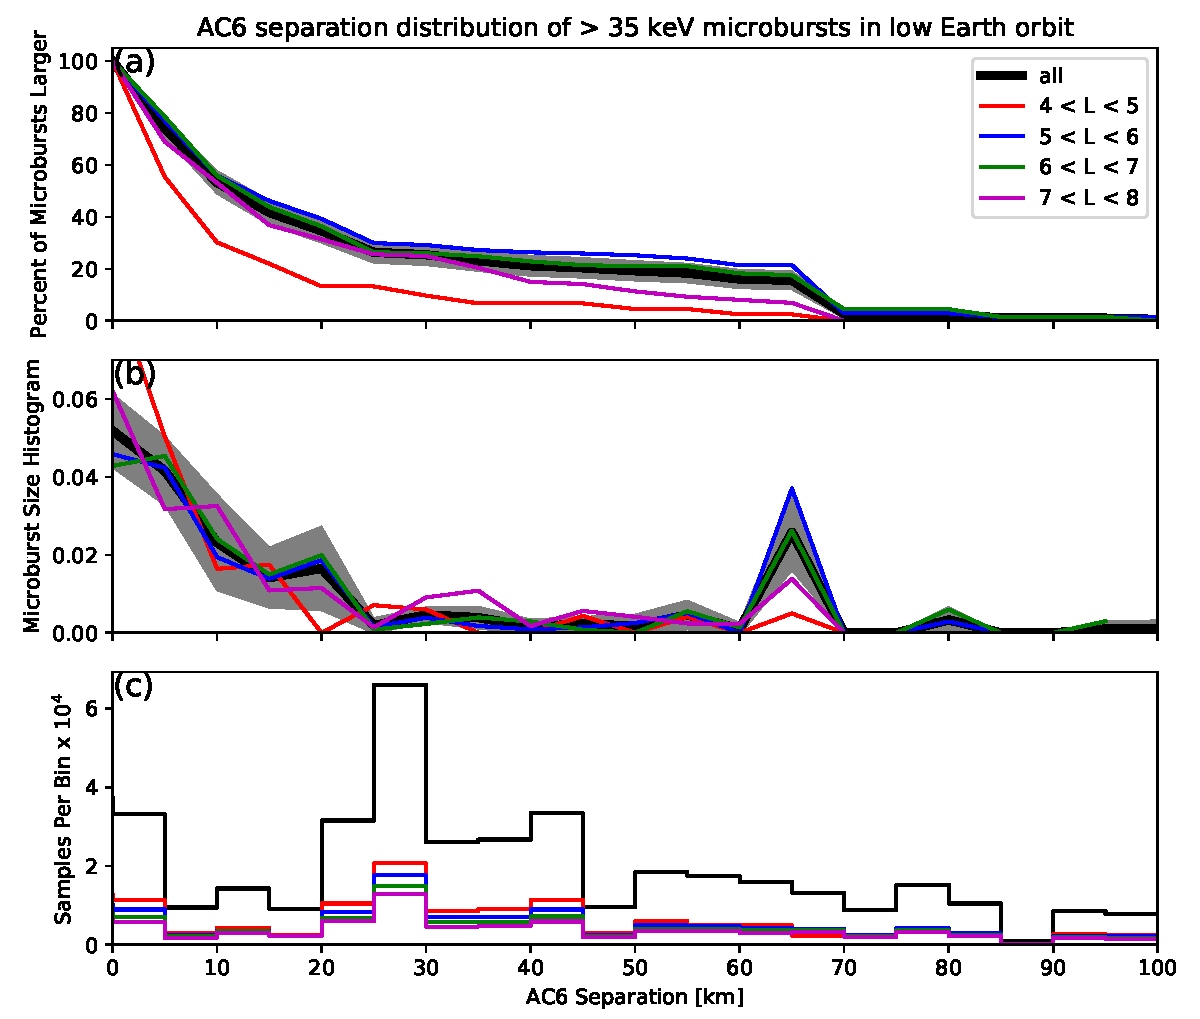
\includegraphics[width=\textwidth]{4_fig3.pdf}
\caption{Microburst size distribution in low Earth orbit. Panel (a) shows the percent of microbursts observed above that separation after normalizing for the uneven AC6 sampling in separation. Panel (b) shows the microburst probability density (size histogram) as a function of separation. Lastly, panel (c) shows the normalization, i.e. number of simultaneous samples AC6 observed as a function of separation. The colored lines show the distributions binned by L, and the thick black curve for the entire radiation belt ($4 < L < 8$). The gray shading around the black curve shows the uncertainty due to counting statistics.}
\label{fig3}
\end{figure}

\begin{figure}
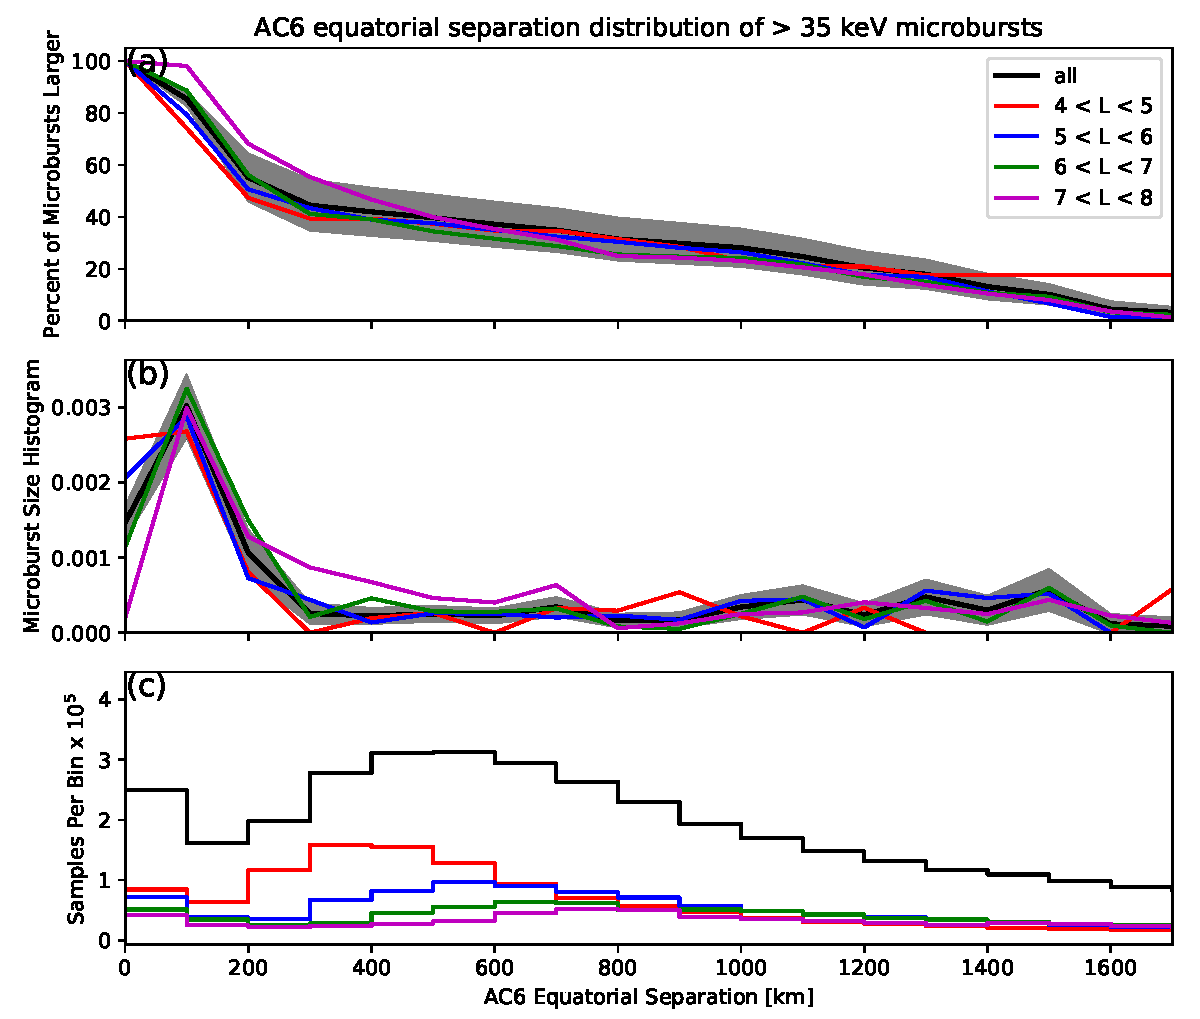
\includegraphics[width=\textwidth]{4_fig4.pdf}
\caption{Microburst size distribution mapped to the magnetic equator in the same format as Fig. \ref{fig3}.} 
\label{fig4}
\end{figure}

\section{Modeling the Distribution of Microburst Sizes} \label{model_section}
\subsection{Monte Carlo and Analytic Models to Calculate $\bar{F}(s)$}

To account for the effects due to microbursts randomly occurring around AC6 with an unknown distribution of microburst sizes, Monte Carlo (MC) and analytic models were developed. These models assume a hypothesized distribution of microburst sizes expressed with a probability density function $p(d | \theta)$ where $\theta$ are the dependent variables, and a microburst footprint shape to estimate $\bar{F}(s)$. The microburst footprint is assumed to be circular with a diameter $d$. $p(d | \theta)$ can be understood as ``the probability of observing a microburst of diameter $d$, given the parameters $\theta$''. Various microburst size distributions were considered: a one-size and two-size microburst populations, and continuous $p(d | \theta)$ such as Maxwell, Weibull, and log-normal.

The Monte Carlo model is the most intuitive. It first randomly scatters $10^5$ microburst centers in a 400 x 400 km grid around AC6. Then each microburst center was assigned a diameter, randomly picked from a $p(d | \theta)$ distribution after $\theta$ parameters were specified. Spacecraft A is placed at the origin, and spacecraft B is placed along the positive y-axis at distances from spacecraft A corresponding to the AC6 separation bins used in Section \ref{microburst_distribution}. Then for each spacecraft B location, the number of microbursts that encompass both spacecraft was counted. The modeled fraction of microbursts observed above $s$ is then

\begin{equation}
\bar{F}(s) = \frac{\displaystyle\sum_{i > s}^\infty n_{i} }{ \displaystyle\sum_{i > 0}^\infty n_{i} }.
\end{equation} where as before the number of microbursts observed by both spacecraft in the ith bin is $n_{i}$.

The analytic model, while identical to the MC model, highlights the geometrical concepts connecting $p(d | \theta)$ and $\bar{F}(s)$ with geometry arguments similar to \citet{Trefall1966}. For a microburst with $d = 2r \geq s$, there is an area between AC6 where that microburst will be observed by both spacecraft if the microburst's center lands there. Figure \ref{fig5}a-c shows this geometry with the two spacecraft indicated with black dots with varying relations between $r$ and $s$. All microbursts who's center lies inside the circular area of radius $r$ surrounding either spacecraft will be observed by that spacecraft. If it exists, the intersection of the two circular areas around both spacecraft defines another area, $A(r, s)$ where a microburst will be observed by both spacecraft if the microburst center lands there. This area can be calculated using the circle-circle intersection area equation, 
\begin{equation}
A(r, s) = 2r^2 \cos^{-1}{\Big( \frac{s}{2r} \Big)} - \frac{s}{2} \sqrt{4r^2 - s^2}.
\end{equation} Example geometries where $A(r, s) > 0$ are shown in Fig. \ref{fig5}b and c. With this conceptual model and $A(r, s)$, the analytic form of $\bar{F}(s)$ can be found and is derived in the Supporting Information (SI) Text S1. To demonstrate the effects of random microburst locations near AC6, examples of the analytic and Monte Carlo $\bar{F}(s)$ curves are shown in Fig. \ref{fig5}d for a one-size, $d=40$ km microburst population.

\begin{figure}
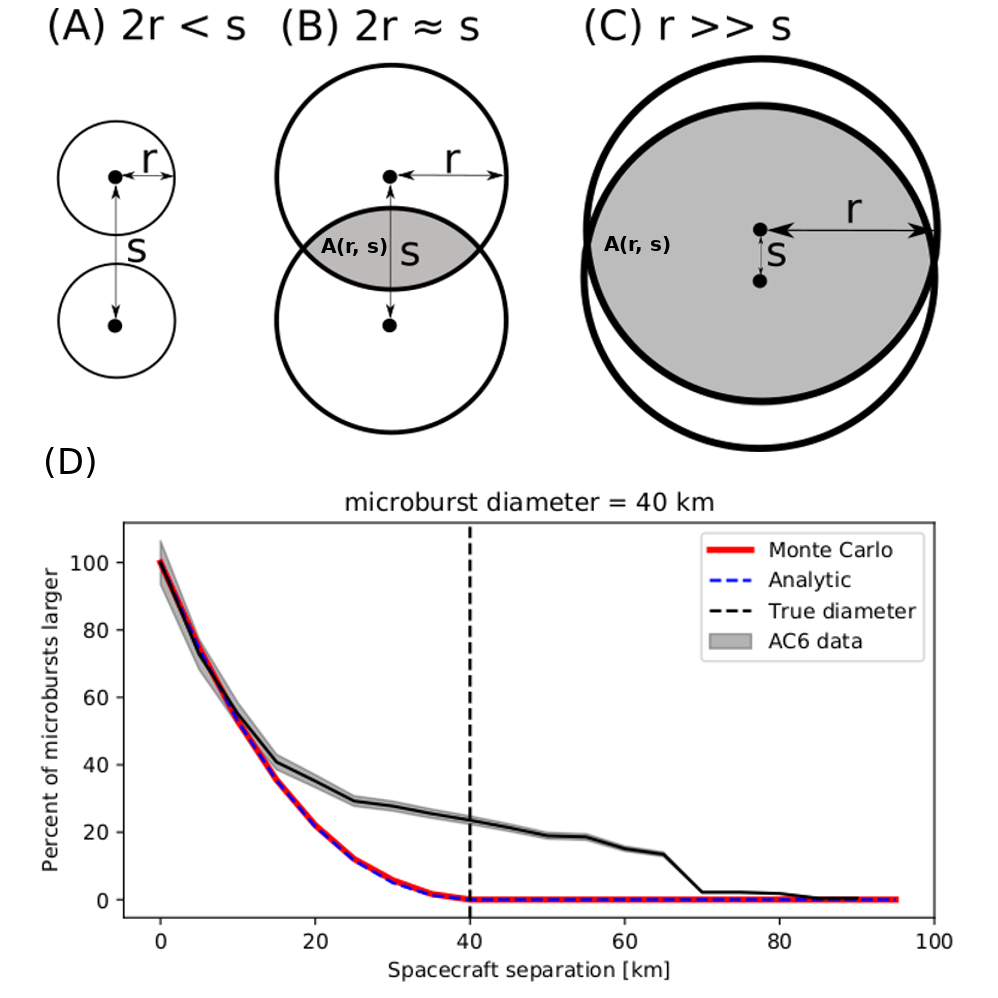
\includegraphics[width=\textwidth]{4_fig5.png}
\caption{Panels A-C show the varying geometries of the analytic model. The two spacecraft are shown as black dots. The enclosing black circle around each spacecraft bounds the area where a microburst will be observed by one or both AC6 units if the microburst's center lies inside the circle. Panel (A) shows the case where microburst diameter is smaller than the AC6 separation and all microbursts will be observed by either unit A or B and never simultaneously. Panel (B) shows the intermediate case where the microburst diameter is comparable to the AC6 separation and some fraction of microbursts will be observed simultaneously. The fraction of the microbursts simultaneously observed is proportional to the circle intersection area $A(r, s)$ and is shown with grey shading. Panel (C) shows the case where the microburst diameter is much larger than the spacecraft separation and nearly all microbursts will be observed by both spacecraft. Lastly panel (D) shows $\bar{F}(s)$ from the AC6 data with a solid black line, and modeled MC and analytic $\bar{F}(s)$ curves for a single-sized microburst distribution with $d = 40$ km.} 
\label{fig5}
\end{figure}

\subsection{Methods for estimating optimal $\theta$ parameters}
At this stage we have all of the ingredients to calculate $\bar{F}(s)$ given a prescribed $p(d | \theta)$. For each $p(d | \theta)$ tested, the optimal $\theta$ parameters are estimated in this study using the traditional least squares regression and Bayesian inference. While we report the $\theta$ parameters that minimize least squares, this section focuses on Bayesian inference because it seamlessly incorporates statistical uncertainty in the data. The uncertainty in the data is then propagated to $\theta$ which is then no longer an optimal value, rather a distribution of values that is consistent with the observations and its uncertainty. 

Bayesian inference is rooted in Bayes theorem of conditional probability. Given the observed $\bar{F}(s)$ as $y$, and model's dependent variables as $\theta$, Bayes theorem can be written as

\begin{equation}
p(\theta | y) = \frac{p(y | \theta) p(\theta)}{p(y)}.
\end{equation} $p(\theta)$ is the distribution of $\theta$ that describe our prior level of knowledge about that parameter e.g. from earlier microburst size studies, a microburst size must less than $500$ km in LEO. This is called the prior which is quantified by a PDF such as normal, uniform, etc. Next term is the likelihood, $p(y | \theta)$, the conditional probability of obtaining $y$ given a particular $\theta$. The likelihood probability is a probabilistic penalty function that quantifies the discrepancy between the modeled and observed $\bar{F}(s)$ in terms of the standard error. The resulting PDF of $\theta$s consistent with the observations is $p(\theta | y)$ known as the posterior distribution. The posterior is an update to our prior distributions, modified by the likelihood i.e. the data and its uncertainties. Here, the posterior is used to make inferences regarding the range of $\theta$ parameters that generate a $\bar{F}(s)$ that is consistent with the observations. The last parameter in Bayes theorem is $p(y)$. $p(y)$ is the marginal likelihood (evidence) that describes the probability of obtaining $y$ after marginalizing over all prior variables. Calculation of $p(y)$ is difficult, and often not necessary for model parameter estimation. 

With all of the above terminology, the important takeaway is that the posterior distribution for each model parameter is interpreted as the range of our model's dependent parameters that are consistent with the observations. A 95\% credible interval (CI) for each model parameter is reported here that is interpreted as: assuming a hypothesized $p(d | \theta)$, there is a 95\% probability that the true $\theta$ is inside the CI. To sample the posterior distribution, the $\theta$ parameter space is explored with a Markov Chain Monte Carlo (MCMC) sampler. In a nutshell a Markov Chain is a process that samples random variables that depend on only the previous state of those random variables. Hence a MCMC sampler is a Monte Carlo sampler that samples the $\theta$ parameter space by picking random $\theta$ values based on the previous state of $\theta$. 

The first and one of the most popular MCMC is the Metropolis-Hastings sampler \citep{Metropolis1953, Hastings1970}. While the Metropolis-Hastings sampler is explained in detail in \citet{Metropolis1953} and \citet{Hastings1970} and a good introduction given in \citet{Sambridge2006} as well as \citet{Sharma2017}, a brief overview is warranted. The Metropolis-Hastings sampler samples the posterior distribution in $N$ trials. Once an initial set of $\theta$ is randomly picked from the prior, the i$^{th}$ trial involves the following steps. First calculate the posterior probability for $\theta_i$. Then pick a proposal $\theta_{i+1}$ to jump to, randomly picked near $\theta_i$ in parameter space. If the $\theta_{i+1}$ posterior probability is higher than $\theta_i$, the MCMC accepts the proposal and moves to $\theta_{i+1}$. If the posterior probability of $\theta_{i+1}$ is smaller than $\theta_{i}$, there is a random chance that $\theta_{i+1}$ will be accepted or rejected (if rejected, $\theta_{i+1} = \theta_i$ and a new proposal is generated). This accept/reject criteria allows the sampler to trend to more probable $\theta$ while also exploring the neighboring regions. After the $N$ trials, a histogram is made using the accepted $\theta$s to produce the posterior distribution for each model parameter.


\subsection{Estimating optimal parameters for various microburst size models}
The MCMC sampler is first used to test the simplest microburst size model where all microbursts are one size and the MCMC will estimate that size. The microburst size PDF for this model can be expressed as
\begin{equation}
p(d | d_0) = \delta(d-d_0)
\end{equation} where $\delta$ is the Dirac Delta function and $d_0$ is the diameter of all microbursts according to this model. The range of $d$ that are consistent with the observed $\bar{F}(s)$ is shown in Fig. \ref{fig6}. Assuming this model, there is a $95 \%$ probability that the microburst diameter is between 38 and 129 km. As a sanity check the optimal size that minimizes least squares is 73 km.

A slight generalization of the one-size model is a two-size microburst population model that assumes the following microburst PDF
\begin{equation}
p(d | d_0, d_1, a) = a \delta(d-d_0) + (1-a)\delta(d-d_1)
\end{equation} where the diameters of the two microburst populations are given by $d_0$ and $d_1$ and $a$ is the parameter that quantifies the relative fractions of the two populations. The result of this model is shown in Fig. \ref{fig7}. The fit is slightly better than the one-size model, although that is to be expected given two more free model parameters. A majority, $98$ \%, of microbursts, have a diameter between $12$ and $47$ km with a rare population with a diameter between $76$ and $234$ km. The set of parameters that minimize least squares is $99.5$ \% of microbursts are small with a size of $21$ km and the remaining $0.5$ \% of microbursts have a $140$ km size.

Other, continuous PDFs were tested including: Maxwellian (Maxwell -- Boltzmann), log-normal, and Weibull. The range of model parameters that are consistent with the observed $\bar{F}(s)$ are presented in the SI text S2. These distributions were chosen because they have the following properties that are most realistic: they are continuous, approach 0 in the limit as $r \rightarrow 0$ (lower bound microburst size is ultimately limited by the electron gyroradius), and can be symmetrical or asymmetrical.

\begin{figure}
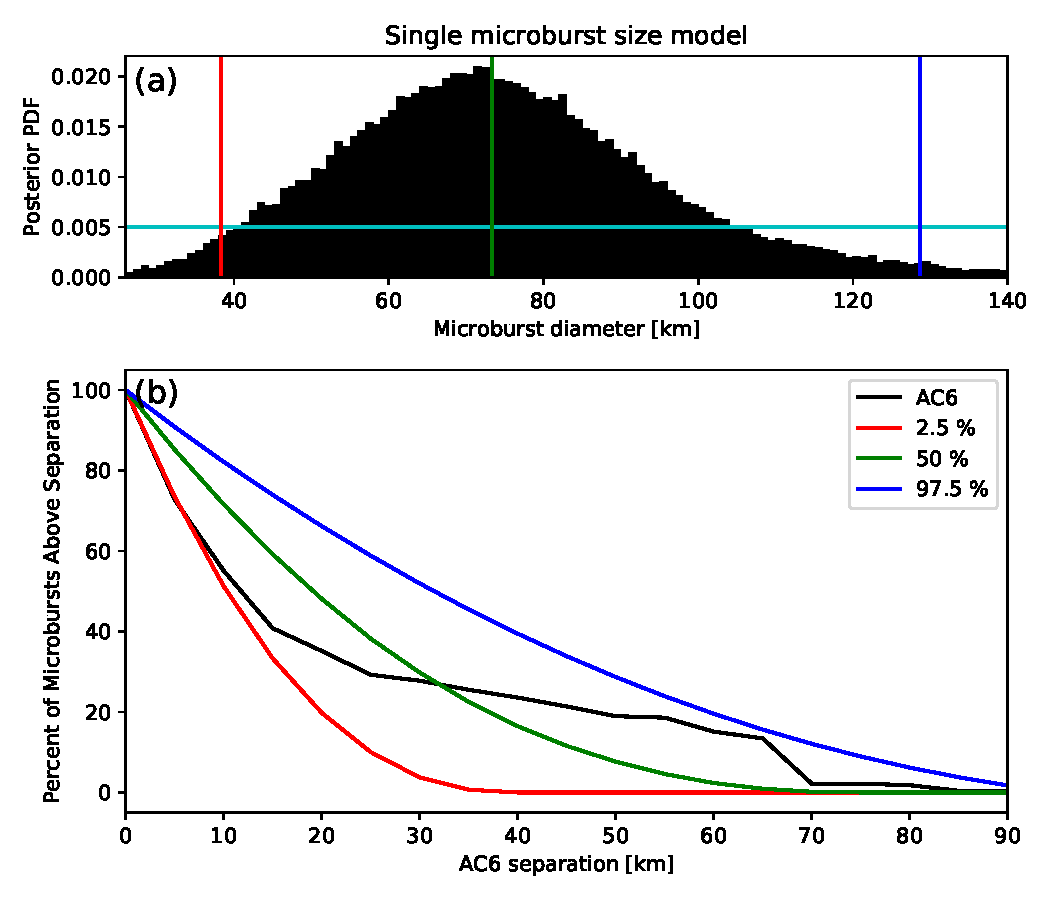
\includegraphics[width=\textwidth]{4_fig6.pdf}
\caption{Range of plausible microburst sizes assuming all microbursts are one fixed size. Panel (a) shows the posterior probability density function of microburst diameters in black. The red, green, and blue vertical lines at 38, 73, and 129 km represent the 2.5, 50, and 97.5 posterior percentiles, respectively. A uniform prior between 0 and 200 km was assumed for this MCMC run and is shown in cyan. Panel (b) shows the percent of microbursts observed above an AC6 separation for $4 < L < 8$ in black. The 2.5, 50 and 97.5 size percentiles were estimated from the posterior and plotted in red, green, and blue curves, respectively.} 
\label{fig6}
\end{figure}

\begin{figure}
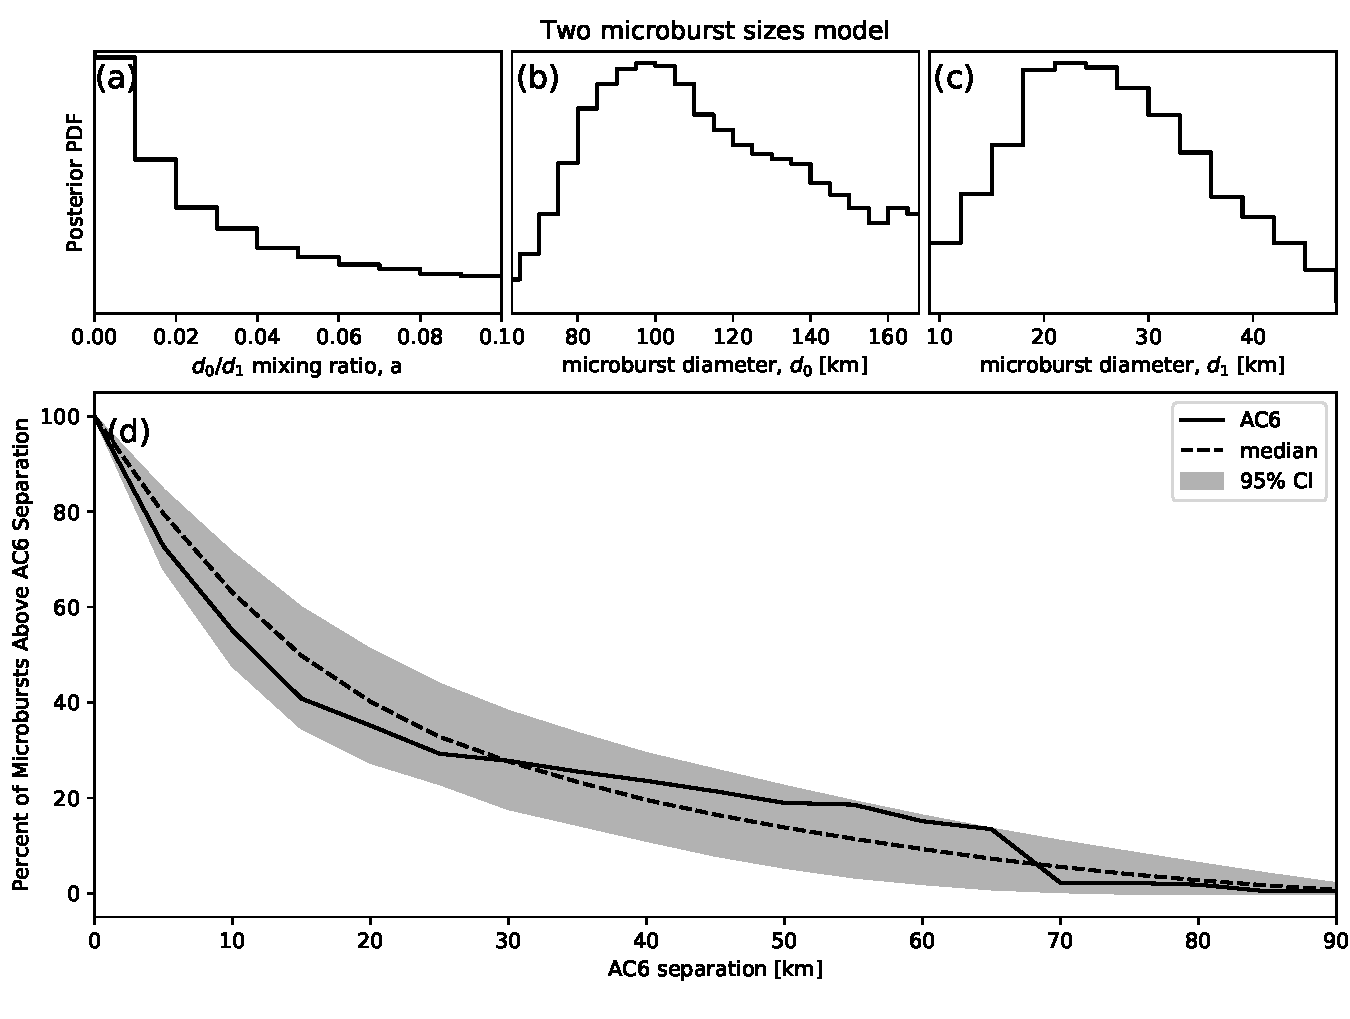
\includegraphics[width=\textwidth]{4_fig7.pdf}
\caption{Plausible microburst percent curves assuming microburst size distribution is bimodal consisting of two sizes $d_0$ and $d_1$ with a mixing term that quantifies the relative occurrence of the $d_0$ to $d_1$ microburst populations. Panel (a) shows the posterior distribution for the microburst population mixing term, $a$ with a median value of $0.02$. The $a$ prior was uniform between 0 and 0.2. Panel (b) shows the posterior distribution for $d_0$, the larger microburst population estimated with a uniform prior between 50 and 200 km and the posterior median diameter of $122$ km. Panel (c) shows the posterior distribution for $d_1$, the smaller microburst population, estimated using a uniform prior between 0 and 50 km with a median diameter of $28$ km. Panel (d) is similar to Fig. \ref{fig6}b and shows the AC6 microburst fraction for $4 < L < 8$ in black. A set of 1000 random parameter triples ($a$, $d_0$, and $d_1$) were drawn from the posterior and used to generate a family of $\bar{F}(s)$ curves. At each $s$ the range of consistent $\bar{F}(s)$ were quantified by the 2.5, 50 and 97.5 percentiles and shown with the red, green, and blue curves, respectively.} 
\label{fig7}
\end{figure}

\section{Discussion} \label{discussion}
The LEO microburst $\bar{F}(s)$ estimated in section \ref{microburst_distribution} shows that a majority of coincident microbursts were observed by AC6 when they were separated by less than a few tens of km. This conclusion is consistent with prior literature and most similar to \citet{Parks1967} who reported that many $> 15$ keV microbursts are less than $40$ km in diameter while others were on average $80 \pm 28$ km in diameter. Furthermore, these results are similar to the bouncing packet example shown in \citet{Blake1996} with a size of ``at least a few tens of kilometers". The relatively small number of large $> 70$ km microbursts observed by AC6 fit in well with the results from \citet{Barcus1966} and \citet{Brown1965_2}, although the AC6 separation is mostly latitudinal while \citet{Barcus1966} and \citet{Brown1965_2} used data from pairs of balloons separated predominantly in longitude. 

Without knowledge of the microburst shape, a direct comparison between the AC6 and balloon observations is difficult. \citet{Trefall1966} discussed how a hypothetical circular microburst at the scattering location near the magnetic equator will be stretched into an ellipse with a semi-major axis in the longitudinal direction. This stretching effect should be explored further as it introduces an ambiguity from the eccentricity of the ellipse that prevents a direct latitudinal and longitudinal comparison.

When comparing our results to more recent studies, the AC6 microburst size distribution is much larger than the sizes reported in \citet{Dietrich2010} who used very low (VLF) frequency transmission paths and SAMPEX to conclude that microbursts must be smaller than 4 km from a small number of microbursts observed during one SAMPEX radiation belt pass. \citet{Dietrich2010} arrived at their conclusion by looking for temporal coincidence of microbursts and FAST events, subsecond VLF transmission perturbations, but the connection between FAST events and microbursts is not well understood. Lastly, our results are consistent with FIREBIRD-II observations of a $> 11$ km microburst reported by \citet{Crew2016}, and the minority of microbursts observed by AC6 up to $s \approx 70$ km are consistent with the $> 51$ km bouncing packet microburst reported in \citet{Shumko2018a}.

The microburst PDF shown in Fig. \ref{fig3}b suggests that the microburst size distribution is bimodal. This has been suggested before by \citet{Blake1996} who noted that the $> 150$ keV and $> 1$ MeV microbursts are not always well correlated e.g. Fig. 10 in \citet{Blake1996}. The quality of the AC6 data is insufficient to definitively conclude that there are two distinct microburst populations. The different microburst population hypothesis can be better tested with an AC6-like mission with better energy resolution and homogeneous MLT coverage.

The model results from section \ref{model_section} emphasize that care must be taken when comparing the $\bar{F}(s)$ curves observed by AC6 and the true microburst size distribution due to the compounding effect of an unknown microburst size distribution, unknown microburst shape, and random microburst locations near AC6. By assuming there is only one microburst size, the results in Fig. \ref{fig6} suggest that there is a 95\% probability that the microburst diameter is somewhere between 38 and 129 km, a relatively wide range of values. On the other hand, the two-size model has a smaller variance around the AC6 $\bar{F}(s)$, which is expected with the addition of two more free parameters. The two size model is interpreted as 98\% of microbursts diameters are between 12 and 47 km and larger microbursts are very uncommon. 

A variety of continuous $p(d)$ such as the Maxwellian, Weibull and log-normal were also tested. While the continuous microburst PDFs are more realistic, there is no clear choice of which microburst PDF nature prefers. The one and two-size model are simple to interpret, and the two-size model qualitatively fits the observations the best out of all $p(d)$ tested. Surely nature does not only have two discrete microburst sizes. Rather, the current evidence and reasoning supports a bimodal and continuous PDF hypothesis. Due to lack of prior observations and theoretical predictions, it is difficult to identify and test a more appropriate $p(d)$ hypothesis at this time.

The equatorial microburst $\bar{F}(s)$ estimated in section \ref{microburst_distribution} and Fig. \ref{fig4}b in particular shows that the majority of microbursts were observed when the equatorial AC6 separation was less than $200$ km. We will now explore how these results compare to prior multi-point measurements of chorus source sizes made near the magnetic equator. The International Sun-Earth Explorers (ISEE 1 and 2) were used by \citet{Gurnett1979} to make one of the first direct chorus source scale measurements. \citet{Gurnett1979} estimated that the wave power correlation scale was on the order of a few hundred km across the background magnetic field. Using the Cluster Wide Band Data measurements \citet{Santolik2003} found the correlation scale of whistler mode chorus waves to be around 100 km near the source region at $L \approx 4$ and midnight MLT sector. Furthermore, \citet{Turner2017} used the four satellites comprising the Magnetospheric Multiscale Mission and found that rising tone whistler mode chorus elements were phase coherent up to 70 km at $L \approx 8$. Lastly, \citet{Agapitov2010, Agapitov2011b, Agapitov2017a, Agapitov2018} used multiple sets of spacecraft missions with wave measurements near the chorus source region to statistically show that the extent of chorus source region can extend from 600 km in the outer radiation belt to greater than 1,000 km in the outer magnetosphere.

The equatorial microburst size of less than a few hundred km shows that the waves responsible for scattering microburst electrons must have correlated properties on those scales. The wave properties necessary for scattering microburst electrons e.g. coherence, polarization, wave normal angle, etc. can be identified by studying the waves properties that are only observed by multiple equatorial spacecraft at small separations. These properties can then aid wave-particle scattering model development by constraining the wave properties and scattering modes responsible for scattering microburst electrons. In turn, future models could then make predictions regarding the distribution of microburst sizes in LEO. 

\section{Conclusions}
In conclusion, the twin AC6 CubeSats enabled the detailed statistical study of microburst sizes from a two point measurement platform. Roughly $60 \%$ of the $> 35$ keV microbursts were simultaneously observed while AC6 was separated by less than $20$ km and the rest were observed up to $\approx 70$ km separation. Modeling the microburst cumulative distribution function is essential to quantify the relationship between the number of microbursts observed as a function of separation to a hypothesized microburst size distributions. The AC6 microburst data, together with modeling, has hinted at the existence of a bimodal microburst size PDF with the majority of microbursts with a diameter smaller than $40$ km and a rare microburst population with a diameter around $100$ km. The bimodal size hypothesis may be more comprehensively addressed from LEO spacecraft with more simultaneous microburst observations, homogeneous MLT coverage, and differential energy channels. Moreover, to disentangle the compounding effect that affects two-point microburst measurements, a X-ray imager on a high altitude balloon can observe the atmospheric microburst footprint and determine the microburst size, shape, and any spatial correlations with little ambiguity. 

When mapped to the magnetic equator, most microbursts were observed while the mapped AC6 separation was less than $200$ km. This correlates well with the sizes of highly correlated chorus waves and it suggests that the wave properties crucial for scattering microbursts must be correlated over relatively small regions. By studying the wave properties that are correlated on a few hundred km scales, the dominant wave scattering modes may be identified.

\section{Acknowledgments}
This work was made possible with the help from the many engineers and scientists at The Aerospace Corporation who designed, built, and operated AC6. M. Shumko was supported by NASA Headquarters under the NASA Earth and Space Science Fellowship Program - Grant 80NSSC18K1204. D.L. Turner is thankful for support from the Van Allen Probes mission and a NASA grant (Prime award number: 80NSSC19K0280). \textcolor{red}{Other Aerospace and MSU funding sources...} The AC6 data is available at http://rbspgway.jhuapl.edu/ac6 and the IRBEM-Lib version used for this analysis can be downloaded from https://sourceforge.net/p/irbem/code/616/tree/.

% REFERENCES
\bibliographystyle{apalike} % Use a style you and your adviser like. abbrv
\references  %do not change this

\end{document}
